%versi 2 (8-10-2016)\chapter{Landasan Teori}
\chapter{Dasar Teori}
\label{chap:teori}

\section{Privasi}
\label{sec:privasi}
Privasi adalah suatu keadaan dimana kehidupan pribadi seseorang atau sekelompok orang terbebas dari pengawasan atau gangguan orang lain. Privasi juga dapat berarti kemampuan satu atau sekelompok individu untuk menutupi atau melindungi kehidupan dan urusan personalnya dari publik dengan mengontrol sumber-sumber informasi mengenai diri mereka. Untuk melakukan publikasi data dari satu perusahaan ke perusahaan lain, digunakan teknik anonimisasi data untuk melindungi dan menyamarkan atribut sensitif untuk setiap data.

\par \textit{Personally Identifiable Information} (PII) adalah standar yang digunakan untuk menentukan apakah informasi yang ada dapat melakukan identifikasi entitas individu secara lansung atau tidak langsung. PII menjelaskan bahwa identifikasi entitas secara langsung dapat dilakukan menggunakan atribut sensitif. Sedangkan identifikasi entitas secara tidak langsung dapat dilakukan menggunakan penggabungan beberapa atribut non-sensitif. PII adalah atribut  yang biasanya terjadi pelanggaran data dan pencurian identitas. Jika data perusahaan atau organisasi terungkap, maka sangat mungkin data pribadi seseorang akan terungkap. Informasi yang diketahui dapat dijual dan digunakan untuk melakukan pencurian identitas, menempatkan korban dalam risiko.
\\\\
Berikut adalah contoh informasi yang bersifat sensitif menurut standar PII:

\begin{itemize}
\item Identitas diri \\ 
Nama lengkap, tempat tanggal lahir, alamat rumah, alamat email.
\item Nomor identitas diri \\
NIK, nomor passport, nomor SIM, nomor wajib pajak, nomor rekening, nomor telepon, dan nomor kartu kredit.
\item Karakteristik pribadi  \\
Foto diri, sidik jari, dan tulisan tangan.
\item Data biometrik \\
Pemindaian retina, jenis suara, dan geometri wajah.
\item Aset informasi lainnya \\
IP Address dan Media Access Control (MAC). 
\end{itemize}

\noindent Berikut adalah contoh informasi yang bersifat non-sensitif menurut standar PII:
\begin{itemize}
\item Rekaman medis
\item Riwayat pendidikan
\item Riwayat pekerjaan 
\item Informasi finasial
\item Letak geografis
\end{itemize}

\newpage
\section{Data Mining}
Data yang dikumpulkan bertambah banyak, sehingga perlu adanya cara untuk melakukan proses ekstraksi informasi pada sekumpulan data yang sangat banyak. Menurut Gartner, \textit{data mining} adalah proses menemukan korelasi, pola, dan tren baru yang bermakna dengan menyaring sejumlah besar data yang disimpan menggunakan teknologi pengenalan pola serta teknik statistik dan matematika. \textit{Data mining} merupakan bagian dari \textit{Knowledge Discovery in Databases} (KDD). KDD adalah proses transformasi sekumpulan data yang disimpan pada basis data menjadi informasi yang berguna.\\

\begin{figure}[H]
	\centering
	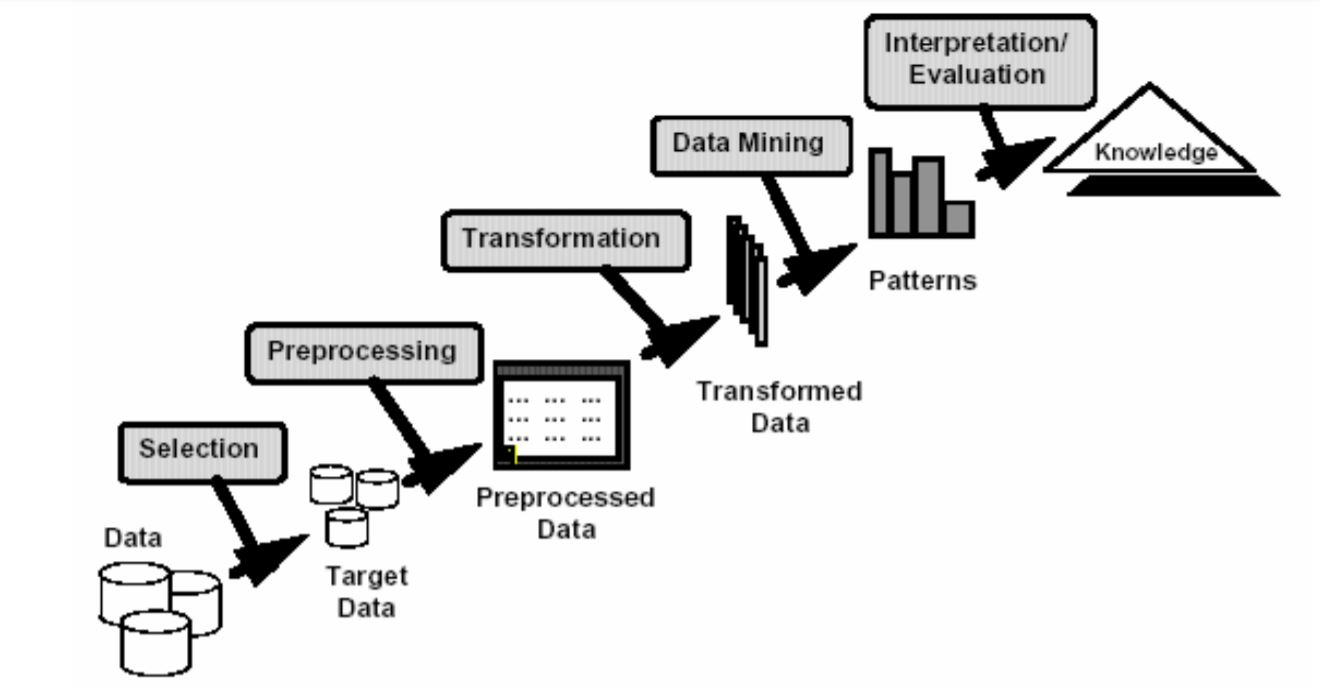
\includegraphics[scale=0.3]{datamining1}
	\caption{Tahapan pada KDD}
	\label{fig:datamining1}
\end{figure}

\noindent Berikut ini adalah penjelasan tahapan pada KDD pada Gambar \ref{fig:datamining1} sebagai berikut:

\begin{enumerate}
\item \textit{Selection}: proses mengambil data yang relevan terhadap analisis.
\item \textit{Preprocessing}: proses pembersihan data dari data yang tidak konsisten dan integrasi data saat penggabungan data.
\item \textit{Transformation}: proses manipulasi data menggunakan konsep agregasi, generalisasi, normalisasi, dan reduksi untuk kebutuhan analisis.
\item \textit{Data mining}: proses ekstraksi informasi menggunakan metode pengenalan pola seperti klasifikasi, pengelompokan/\textit{clustering}.
\item \textit{Interpretation/evaluation}: proses interpretasi hasil pengolahan data menjadi sebuah grafik yang dapat dimengerti.
\end{enumerate}


\noindent Berikut adalah beberapa jenis tipe data terkait teknik data mining:

\begin{itemize}

\item \textit{Binary}: tipe data alphabet/numerik yang hanya memiliki 2 kemungkinan nilai.\\
Contoh: diadakan survei evaluasi beberapa produk pakaian untuk mengetahui produk yang diminati dan tidak diminati. Penilaian produk dapat diwakilkan nilai True atau False. True atau False termasuk jenis binary.

\item \textit{Nominal}: tipe data alphabet/numerik yang memiliki lebih dari 2 kemungkinan nilai.\\
Contoh: seseorang memilih beberapa bahan dari warna yang berbeda. Warna yang mungkin adalah kuning, hijau, hitam, merah. Warna termasuk jenis nominal.

\end{itemize}

\noindent Tujuan dari penggunaan teknik \textit{data mining} adalah sebagai berikut:

\begin{itemize}

\item Prediksi: proses menggunakan nilai dari beberapa atribut yang sudah ada untuk memprediksi nilai atribut di masa yang akan datang. Contoh: klasifikasi.

\item Deskripsi: proses menemukan pola yang dapat merepresentasikan kelompok dari sebuah data. Contoh: pengelompokan/\textit{clustering}.

\end{itemize}

\subsection{Klasifikasi} 
Klasifikasi adalah proses menemukan model (atau fungsi) yang cocok untuk mendeskripsikan dan membedakan sebuah kelas data dengan kelas data lain. Dalam pembelajaran mesin, klasifikasi sering dianggap sebagai contoh dari metode pembelajaran yang diawasi, yaitu menyimpulkan fungsi dari data pelatihan berlabel.\\

\noindent Berikut adalah tahapan klasifikasi secara umum:
\begin{enumerate}

\item
Pelatihan: proses konstruksi model klasifikasi menggunakan algoritma tertentu. Algoritma digunakan untuk membuat model belajar menggunakan set pelatihan data yang tersedia. Model dilatih untuk menghasilkan prediksi yang akurat.

\item
Klasifikasi: model yang digunakan untuk memprediksi label kelas dan menguji model yang dibangun pada data uji dan karenanya memperkirakan akurasi aturan klasifikasi.
\end{enumerate}
\vspace{0.3cm}
\noindent Berikut adalah kategori pemodelan klasifikasi:
\begin{itemize}

\item 
\textit{Discriminative}: pemodelan paling mendasar untuk menentukan satu kelas untuk setiap baris data. Pemodelan ini bergantung pada data yang diamati dan sangat bergantung pada kualitas data daripada distribusi data.

\begin{figure}[H]
	\centering
	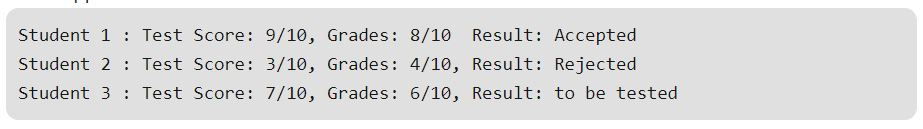
\includegraphics[scale=0.75]{klasifikasi1}
	\caption{Contoh Logistic Regression}
	\label{fig:klasifikasi1}
\end{figure}

Contoh: \textit{Logistic Regression}\\
Gambar \ref{fig:klasifikasi1} adalah penerimaan siswa pada sebuah Universitas, untuk mempertimbangkan \textit{test score} dan \textit{grades} terhadap keputusan seorang siswa diterima/tidak diterima.

\item 
\textit{Generative}: pemodelan ini memodelkan distribusi kelas individu dan mencoba mempelajari model yang menghasilkan data dengan memperkirakan asumsi dan distribusi model. Digunakan untuk memprediksi nilai data yang belum diketahui. \\\\
Contoh: \textit{Naive Bayes} \\
Mendeteksi email spam dengan melihat data sebelumnya. Misalkan dari 100 email yang ada dibagi menjadi kategori Kelas A: 25\% (Email spam) dan Kelas B: 75\% (Email Non-Spam). Ingin diperiksa apakah email berisi  spam atau bukan. Pada Kelas A, 20 dari 25 email adalah spam dan sisanya bukan spam. Pada Kelas B, 70 dari 75 email bukan spam dan sisanya adalah spam. Probabilitas email yang berisi spam termasuk pemodelan \textit{naive bayes}. \\
\end{itemize}

\noindent Berikut adalah contoh pemodelan yang umum digunakan:
\begin{itemize}
\item \textit{Decision Trees}
\item \textit{Naive Bayes}
\item \textit{Neural Networks}
\item \textit{K-Nearest Neighbour}
\item \textit{Linear Regression}
\end{itemize}

\newpage
\subsection{Naive bayes}
\label{sec:naive_bayes}
\par \textit{Naive Bayes} menerapkan klasifikasi dengan menggunakan metode probabilitas dan statistik. Pemodelan ini mencari nilai probabilitas tertinggi pada masing-masing kelas menggunakan teorema \textit{Bayes}. Kelas dengan probabilitas tertinggi akan dipilih sebagai hasil akhir. \textit{Naive Bayes} mudah untuk dibangun dan memiliki komputasi yang lebih cepat daripada model klasifikasi lainnya.\\

\noindent Teorema \textit{Bayes} menemukan probabilitas suatu peristiwa terjadi mengingat probabilitas peristiwa lain yang telah terjadi. Teorema \textit{Bayes} dinyatakan secara matematis melalui persamaan berikut:

\begin{equation}
P(H|D) = \frac{P(D|H) \cdot P(H)}{P(D)}
\end{equation}

\noindent
Dari perhitungan probabilitas teorema Bayes, akan dicari kelas dengan probabilitas maksimum. Probabilitas maksimum dapat dinyatakan secara matematis melalui persamaan berikut:

\begin{align}
MAP(H) = max(P(H|D))
\end{align}

\noindent Keterangan:
\begin{itemize}
\item P(H|D) adalah probabilitas posterior apabila diberika hipotesis H dan diketahui data D. 
\item P(D|H) adalah probabilitas posterior data D jika hipotesis h adalah benar.
\item P(H) adalah probabilitas hipotesis h adalah benar 
\item P(D) adalah probabilitas data.
\end{itemize}

\vspace{0.3cm}

\noindent Gambar \ref{fig:naive_bayes1} diberikan untuk menggambarkan kondisi cuaca saat bermain golf. Masing-masing data dikategorikan berdasarkan nilai atribut \textit{PlayGolf}, yaitu cocok (\textit{Yes}) atau tidak cocok (\textit{No}). 

\begin{figure}[H]
	\centering
	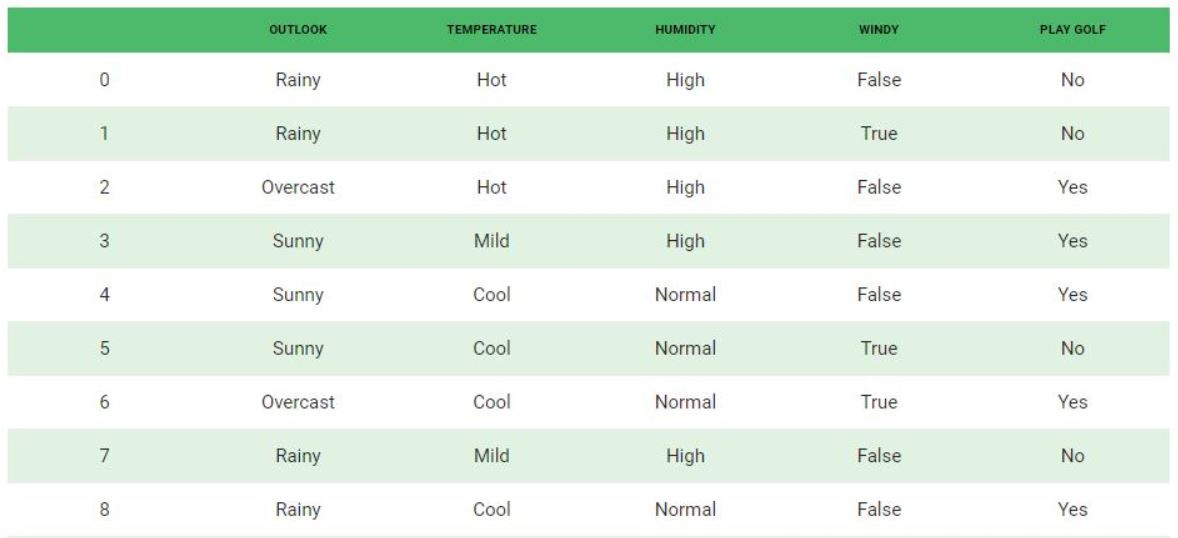
\includegraphics[scale=0.75]{naive_bayes1}
	\caption{Dataset Kondisi Cuaca Bermain Golf}
	\label{fig:naive_bayes1}
\end{figure}

\noindent Berikut adalah pengelompokan nilai berdasarkan dataset yang telah diberikan:

\begin{itemize}

\item 
Vektor fitur\\
Vektor fitur adalah vektor yang mewakili nilai fitur untuk setiap baris dataset. Vektor fitur dalam dataset ini tersusun dari nilai atribut \textit{Outlook, Temperature, Humidity, dan Windy}.

\item
Vektor respon\\
Vektor respon adalah nilai prediksi kelas untuk setiap vektor fitur. Vektor Respon dalam dataset ini diwakili oleh nilai atribut \textit{PlayGolf}.

\end{itemize}


\noindent Secara singkat, langkah kerja algoritma \textit{Naive Bayes} dapat dijelaskan sebagai berikut:

\begin{enumerate}
\item Merepresentasikan teorema Bayes terhadap vektor fitur.\\
Berdasarkan dataset, teorema Bayes dapat diubah seperti berikut:

\begin{equation}
P(y|X) = \frac{P(X|y) \cdot P(y)}{P(X)}
\end{equation}

Di mana y adalah variabel kelas dan X adalah vektor fitur (dengan ukuran n), dinyatakan melalui persamaan berikut:

\begin{equation}
X = (x_1, x_2, x_3, \ldots, x_n)
\end{equation}

Contoh: X = (Rainy, Hot, High, False), y = No
\\\\
Diasumsikan teorema \textit{Bayes} saling independen terhadap fitur-fiturnya. Berikut adalah persamaan teorema \textit{Bayes} baru, jika memakai lebih dari satu nilai atribut:

\begin{equation}
P(y|x_1,\ldots,x_n) = \frac{P(x_1|y) P(x_2|y) \ldots P(x_n|y) P(y)}{P(x_1) P(x_2) \ldots P(x_n)}
\end{equation}


\item Gambar \ref{fig:naive_bayes2} adalah contoh menghitung probabilitas masing-masing atribut.

\begin{figure}[H]
	\centering
	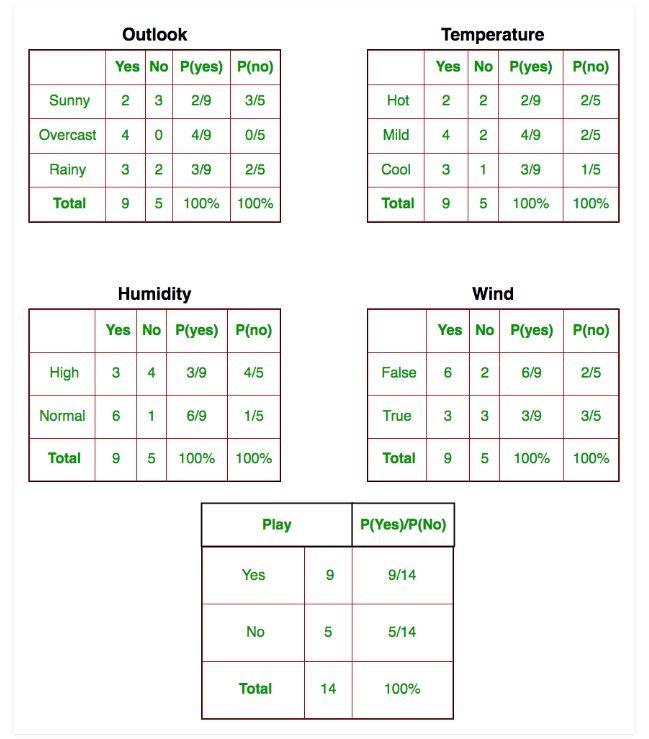
\includegraphics[scale=0.55]{naive_bayes2}
	\caption{Menghitung Probabilitas}
	\label{fig:naive_bayes2}
\end{figure}

Contoh: menghitung $P(No)$ untuk nilai \textit{Sunny} pada atribut \textit{Outlook}
\begin{equation}
P(No) = \frac{frekuensi(Sunny \cap No)}{frekuensi(No)}
\end{equation}

Contoh: menghitung $P(Yes)$ untuk nilai \textit{Sunny} pada atribut \textit{Outlook}
\begin{equation}
P(Yes) = \frac{frekuensi(Sunny \cap Yes)}{frekuensi(Yes)}
\end{equation}

\item Menghitung probabilitas bersyarat jika diketahui nilai dari data baru. \\\\
Contoh: \textit{today = (Sunny, Hot, Normal, False)}
\begin{figure}[H]
	\centering
	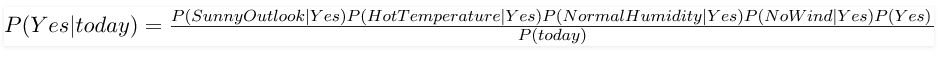
\includegraphics[scale=0.73]{naive_bayes3}
	\label{fig:naive_bayes3}
\end{figure}

\begin{equation}
P(Yes|today) = \frac{3}{5} \cdot \frac{2}{5} \cdot \frac{1}{5} \cdot \frac{2}{5} \cdot \frac{5}{14} = 0.0068
\end{equation}

\begin{figure}[H]
	\centering
	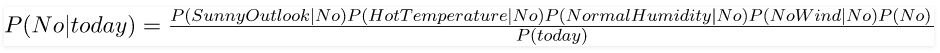
\includegraphics[scale=0.73]{naive_bayes4}
	\label{fig:naive_bayes4}
\end{figure}

\begin{equation}
P(Yes|today) = \frac{2}{9} \cdot \frac{2}{9} \cdot \frac{6}{9} \cdot \frac{6}{9} \cdot \frac{9}{14} = 0.0068
\end{equation}

\item Melakukan normalisasi terhadap probabilitas besyarat.\\

Setelah probabilitas bersyarat dinormalisasi, akan menjadi seperti berikut:

\begin{equation}
P(Yes|today) = \frac{0.0141}{0.0141 + 0.0068} = 0.67
\end{equation}

\begin{equation}
P(Yes|today) = \frac{0.0068}{0.0141 + 0.0068} = 0.33
\end{equation}

Sehingga memiliki probabilitas total seperti berikut:

\begin{equation}
P(Yes|today) + P(No|today) = 1
\end{equation}

\item Mencari probabilitas tertinggi.\\

Berdasarkan pernyataan berikut:
\begin{equation}
P(Yes|today) > P(No|today)
\end{equation}

\noindent Dapat disimpulkan bahwa, jika diberikan data dengan nilai \textit{(Sunny, Hot, Normal, False)} klasifikasi yang tepat untuk atribut \textit{PlayGolf} adalah \textit{Yes}.



\end{enumerate}

\newpage
\subsection{Pengelompokan/Clustering} 
\textit{Clustering} adalah salah satu teknik analisis data yang paling umum digunakan untuk mendapatkan kemiripan antar data. \textit{Clustering} dapat didefinisikan sebagai sebuah tugas untuk mengidentifikasi subkelompok dalam data sedemikian rupa sehingga titik data dalam subkelompok/\textit{cluster} yang sama sangat mirip sedangkan titik data dalam kelompok berbeda sangat berbeda. Contoh pemodelan \textit{clustering} adalah \textit{K-Means}.

\subsection{K-Means} 
\label{sec:k_means}
\textit Algoritma {k-means} adalah algoritma pembelajaran mesin \textit{unsupervised learning} untuk menentukan objek tersebut benar-benar milik kelompok data tertentu. \textit{Unsupervised learning} artinya tidak ada label yang ditentukan dalam data. Gagasan utama \textit{k-means} adalah menetapkan setiap data ke dalam cluster dengan mean terdekat (centroid). Mencari titik terdekat dilakukan dengan cara menghitung distance antara dua data menggunakan Euclidean distance, lalu membandingkat titik yang memiliki jarang paling dekat dengan titik lainnya. \\

\noindent Berikut adalah persamaan untuk menghitung \textit{Euclidean distance}:
\begin{equation}
EuclidDist(p_i,C_i) = \sqrt[]{(p_1-C_1)^2+(p_2-C_2)^2+\ldots +(p_n-C_n)^2}
\end{equation}
\vspace{0.2cm}

\noindent Gambar \ref{fig:kmeans_1} adalah skor A dan B untuk masing-masing individu:

\begin{figure}[H]
	\centering
	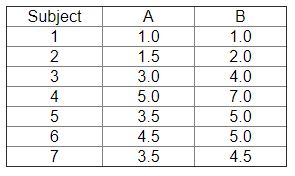
\includegraphics[scale=0.9]{kmeans_1}
	\caption{Contoh Dataset K-Means}
	\label{fig:kmeans_1}
\end{figure}

\noindent Secara singkat, langkah kerja algoritma \textit{k-means} dapat dijelaskan sebagai berikut:
\begin{enumerate}

\item Gambar \ref{fig:kmeans_2} adalah hasil pengelompokan awal untuk k = 2. Untuk menentukan titik centroid awal, akan dicari nilai A dan B terjauh dengan data lainnya menggunakan Euclidean distance.

\begin{figure}[H]
	\centering
	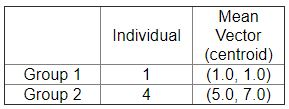
\includegraphics[scale=0.9]{kmeans_2}
	\caption{Hasil Pengelompokan Awal}
	\label{fig:kmeans_2}
\end{figure}

\item Data yang tersisa akan diperiksa secara berurutan dan dialokasikan pada cluster yang paling dekat dengan \textit{centroid} awal menggunakan \textit{Euclidean distance}. Gambar \ref{fig:kmeans_3} menunjukan vektor rata-rata (centroid) akan dihitung ulang setiap kali anggota baru ditambahkan.

\begin{figure}[H]
	\centering
	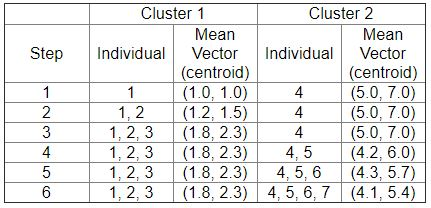
\includegraphics[scale=0.9]{kmeans_3}
	\caption{Mencari Centroid Kelompok}
	\label{fig:kmeans_3}
\end{figure}

\item Menentukan titik \textit{centroid} baru pada \textit{cluster} yang baru terbentuk dari tahap sebelumnya.

\begin{figure}[H]
	\centering
	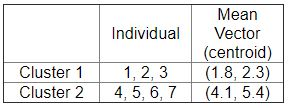
\includegraphics[scale=0.9]{kmeans_4}
	\caption{Hasil Pengelompokan Baru}
	\label{fig:kmeans_4}
\end{figure}

\item Belum bisa dipastikan bahwa setiap individu telah dialokasikan pada cluster yang tepat. Oleh karena itu, perlu membandingkan \textit{distance} masing-masing data dengan \textit{centroid} baru pada masing-masing kelompok. Gambar \ref{fig:kmeans_5} adalah tabel hasil perbandingan \textit{distance} yang dihitung menggunakan rumus \textit{Euclidian distance}.

\begin{figure}[H]
	\centering
	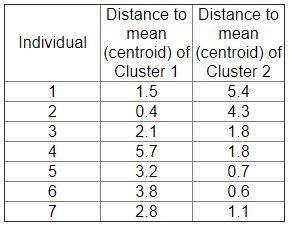
\includegraphics[scale=0.9]{kmeans_5}
	\caption{Euclidean Distance Cluster 1, Cluster 2}
	\label{fig:kmeans_5}
\end{figure}

\item Dapat disimpulkan bahwa, hanya individu 3 yang jaraknya lebih dekat dengan \textit{centroid Cluster 2} dari pada \textit{centroid Cluster 1}. Dengan kata lain, distance masing-masing individu ke centroid kelompoknya sendiri harus lebih kecil daripada rata-rata kelompok lain. Dengan demikian, individu 3 harus dialokasikan ke \textit{Cluster 2}. Gambar \ref{fig:kmeans_6} adalah hasil pengelompokan akhir yang dihasilkan oleh pemodelan \textit{k-means}.

\begin{figure}[H]
	\centering
	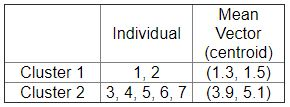
\includegraphics[scale=0.9]{kmeans_6}
	\caption{Hasil Pengelompokan Akhir}
	\label{fig:kmeans_6}
\end{figure}



\end{enumerate}





\newpage
\section{Bidang Terkait Data Mining}
\textit{Data mining} terhubung dengan beberapa bidang lain seperti statistika, \textit{machine learning}, pengenalan pola, sistem basisdata, sistem \textit{data warehouse}, \textit{information retrieval}, visualisasi data, dan bidang lainnya. Jenis bidang ini memberikan berkontribusi yang signifikan terhadap keberhasilan dalam pengolahan data menggunakan teknik \textit{data mining}.

\begin{figure}[H]
	\centering
	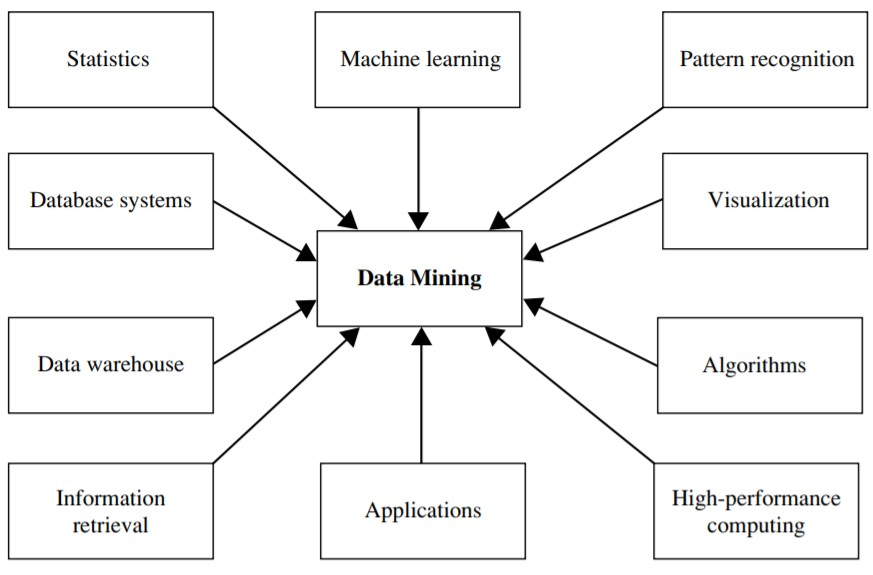
\includegraphics[scale=0.5]{teknologidatamining1}
	\caption{Jenis bidang terkait data mining}
	\label{fig:rnaalgorithm}
\end{figure}

\subsection{Visualisasi Data} 
Visualisasi adalah penggunaan representasi grafik pada komputer. Visualisasi data melibatkan penyajian data dalam bentuk grafik atau gambar agar membuat informasi mudah dimengerti, membantu menjelaskan fakta, dan menentukan arah tindakan.  Dengan adanya representasi data dalam bentuk visual, seseorang dapat memahami sekumpulan data dengan mudah. Hal ini membantu individu  menemukan pola, memahami informasi, dan membentuk opini berdasarkan hasil analisis. 
\\\\
Beberapa teknik visualisasi yang umum digunakan untuk menggambarkan informasi dari sekumpulan data adalah sebagai berikut:

\begin{itemize}
\item \textit{Line chart} adalah grafik pembanding perubahan nilai atribut pada periode waktu tertentu.
\item \textit{Bar chart} adalah grafik pembanding nilai atribut untuk jenis kategori yang berbeda.
\item \textit{Scatter plot} adalah grafik dengan plot dua dimensi yang menunjukkan variasi dua item.
\item \textit{Pie chart} adalah grafik untuk membandingkan persentase nilai atribut secara keseluruhan.
\end{itemize}

\subsection{Statistika}
Statistika adalah pengetahuan yang berkaitan dengan pengumpulan angka-angka, pengolahan, dan analisis, penarikan kesimpulan, dan membuat keputusan berdasarkan data dan fakta yang sudah dianalisis. Analisis yang dilakukan dalam statistika meliputi ukuran pemusatan dan penyebaran data. Ukuran pemusatan data meliputi nilai rata-rata (\textit{mean}), \textit{modus}, dan \textit{median}. Sedangkan ukuran penyebaran data meliputi variansi dan standar deviasi

\subsubsection{Mean}
\textit{Mean} adalah nilai rata-rata dari sekumpulan data. Nilai dari \textit{mean} dapat ditentukan dengan cara membagi jumlah data yang ada dengan total data. \textit{Mean} terdiri dari dua jenis yaitu: populasi dan sampel. Mean populasi memiliki simbol $\mu$, sedangkan \textit{mean} untuk sampel memiliki simbol $\overline{x}$.   
\\\\
Berikut adalah persamaan untuk menghitung \textit{mean} populasi ($\mu$):

\begin{equation}
\mu = \frac{x_1+x_2+x_3+\ldots+x_n}{n}
\end{equation}

\noindent Berikut adalah persamaan untuk menghitung \textit{mean} sampel ($\overline{x}$):

\begin{equation}
\overline{x} = \frac{x_1+x_2+x_3+\ldots+x_n}{n}
\end{equation}


\subsubsection{Median}
\textit{Median} menentukan letak dari titik tengah data setelah data disusun menurut urutan nilainya. \textit{Median} disimbolkan dengan $\widetilde x$. Median dibedakan  berdasarkan jumlah datanya, yaitu jumlah data yang bernilai ganjil dan jumlah data yang bernilai genap. 
\\\\
\noindent Berikut adalah persamaan \textit{median} untuk jumlah data ganjil dan genap:

\begin{align}
\widetilde x = 
\left\{ \begin{array}{cc} 
X_{\frac{n+1}{2}} & \hspace{5mm} ,n=ganjil \vspace{2mm}\\
\frac{X_{\frac{n}{2}}+X_{\frac{n}{2}+1}}{2}  & \hspace{5mm} ,n=genap \\
 \end{array} 
 \right.
\end{align}

\subsubsection{Modus}
\textit{Modus} adalah nilai yang sering muncul dalam kelompok data tersebut. \textit{Modus} berarti nilai data yang memiliki frekuensi terbanyak dalam sekelompok data. 


\subsection{Machine Learning} 
\textit{Machine learning} mempelajari metode pembelajaran pada sebuah komputer, agar dapat belajar secara mandiri atau meningkatkan kinerjanya berdasarkan data pelatihan yang pernah diberi. Penelitian pada \textit{machine learning} adalah membuat program komputer bekerja secara otomatis untuk belajar mengenali pola yang kompleks dan membuat keputusan cerdas berdasarkan data. \\

\noindent Berikut adalah contoh pembelajaran pada \textit{machine learning}:

\begin{itemize}

\item
\textit{Supervised learning} adalah pembelajaran dengan menggunakan data yang diberi label dengan baik yang berarti beberapa data sudah ditandai dengan jawaban yang benar. \textit{Supervised learning} menganalisis data pelatihan dan menghasilkan hasil pelatihan yang benar dari data yang diberi label. Contoh penerapannya adalah \textit{pengelompokan/clustering}.

\item
\textit{Unsupervised learning} adalah pembelajaran menggunakan informasi yang tidak diklasifikasikan atau diberi label dan memungkinkan algoritma  bertindak pada informasi tersebut tanpa bimbingan. \textit{Unsupervised learning} bertujuan untuk mengelompokkan informasi yang tidak disortir menurut persamaan, pola dan perbedaan tanpa pelatihan data sebelumnya. Contoh penerapannya adalah klasifikasi.

\end{itemize}

\newpage
\section{Privacy Preserving Data Mining (PPDM)} 
\textit{Privacy Preserving Data Mining} (PPDM) adalah teknik yang telah dikembangkan untuk mencegah pengungkapan informasi sensitif seseorang saat dilakukan \textit{data mining} dari sekumpulan data yang berukuran besar. PPDM dapat melakukan perubahan dan  menghilangkan sebagian data untuk menjaga privasi. Semakin banyak terjadinya perubahan pada data, maka perlindungan privasi akan meningkat dan kualitas informasi akan menurun. Utilitas adalah kondisi untuk meningkatkan kualitas informasi yang diperoleh dengan mempertimbangkan jumlah data yang dimodifikasi. Metode PPDM menjamin perlindungan data pada tingkat privasi tertentu bersamaan dengan memaksimalkan utilitas data, sehingga memungkinkan pengolahan \textit{data mining} menghasilkan informasi yang efektif. Klasifikasi PPDM dibuat berdasarkan siklus pengolahan data mulai dari pengumpulan data, proses data mining, penerbitan data, dan distribusi data.

\subsection{Pengumpulan Data} 
Untuk memastikan privasi tetap terjada pada saat pengumpulan data, perangkat sensor sebagai reseptor input dapat mengacak nilai data yang ditangkap sebelum data dikirimkan kepada kolektor (perangkat lain). Entitas yang mengumpulkan data diasumsikan menjadi entitas yang tidak dapat dipercaya. Oleh karena itu, nilai-nilai data sesungguhnya tidak pernah disimpan dalam basis data, dan nilai-nilai tersebut hanya dapat digunakan setelah melalui tahap transformasi (saat proses KDD). Metode yang dapat digunakan untuk melindungi atribut sensitif saat pengumpulan data adalah \textit{randomisation}.

\subsection{Proses Data Mining} 
\textit{Data mining} sangat memungkinkan terjadinya identifikasi terhadap atribut sensitif. Berikut adalah beberapa metode yang dapat digunakan untuk melindungi atribut sensitif seseorang saat proses \textit{data mining} yaitu: \textit{association rule hiding} adalah aturan untuk mengekstraksi seluruh atribut non-sensitif, \textit{downgrading classifier effectiveness} adalah teknik untuk menurunkan keakuratan dari \textit{classifier} yang sering digunakan, \textit{query auditing and inference control} adalah aturan yang membatasi lingkup penggunaan kueri agregasi berdasarkan dataset, bukan terhadap catatan individu atau kelompok tertentu.

\subsection{Publikasi Data} 
Ada kondisi di mana sebuah perusahaan ingin melakukan publikasi koleksi data baik secara publik atau kepada pihak ketiga untuk analisis data tanpa mengungkapkan kepemilikan data sensitif. Dalam situasi ini, PPDM dapat dicapai dengan melakukan anonimisasi pada atribut data yang bersifat sensitif sebelum data tersebut dipublikasikan. PPDM pada publikasi data dikenal sebagai \textit{Privacy Preserving Data Publishing} (PPDP). Berikut adalah beberapa metode yang dapat digunakan untuk melindungi atribut sensitif saat publikasi data yaitu: \textit{k-anonymity, l-diversity, t-closeness, e-differential privacy.}

\subsection{Distribusi Data} 
Ada kondisi di mana seseorang berusaha untuk melakukan teknik \textit{data mining} melalui data yang bersifat publik, berdasarkan ketehubungan nilai atribut non-sensitif. Beberapa pendekatan dapat digunakan untuk melindungi atribut sensitif saat distribusi data. Pendekatan pertama adalah menggunakan protokol yang aman untuk mencegah pengungkapan atau perhitungan informasi antar entitas seperti: \textit{oblivious transfer protocol} dan \textit{homomorphic encryption}. Pendekatan kedua adalah mempertimbangkan sekumpulan operasi primitif yang sering digunakan pada algoritma \textit{data mining} seperti: \textit{secure sum, secure set union, secure size of intersection, scalar product and the set intersection}.

\section{Jenis Serangan Publikasi Data} 
Menurut Dalenius (1977), perlindungan privasi tidak akan memberikan kesempatan bagi orang lain untuk mendapatkan informasi sensitif spesifik dari seseorang atau individu meskipun orang lain mengetahui informasi umum yang berhubungan dengan informasi sensitif individu tersebut. Secara umum, orang lain dapat menemukan sebuah cara untuk memetakan sebuah data ke dalam tabel yang telah dianonimisasi ketika data tersebut telah dipublikasikan. Serangan ini dikenal dengan istilah \textit{linkage attack}. Model serangan ini dapat dikategorikan menjadi dua macam, berdasarkan jenis serangannya.

\subsection{\textit{Record Linkage}}
\textit{Record linkage} mengacu pada pemetaan beberapa data korban yang ditargetkan ke dalam sebuah tabel yang dirilis secara publik berdasarkan prinsip anonimisasi. Jika pada proses identifikasi salah satu nilai data cocok dengan nilai data lainnya pada tabel yang sudah dipublikasi, maka memungkinkan atribut sensitif miliki seseorang dapat diketahui oleh orang lain. Menggunakan pemodelan \textit{k-anonimity}, terbukti dapat menghindari jenis serangan \textit{record linkage}.

\subsection{\textit{Attribute Linkage}} 
Dalam serangan ini, penyerang mendapatkan beberapa informasi terkait atribut sensitifnya, meskipun penyerang tidak dapat menghubungkan satu data dengan data lain dari data yang telah dipublikasi. Pemodelan \textit{l-diversity} dapat mencegah serangan attribute linkage. Kondisi yang diperlukan adalah kesetaraan setidaknya sebuah data memiliki l nilai atribut yang berbeda dengan data lainnya pada data yang telah dipublikasi. Konsep dasarnya adalah menghindari hubungan atribut jika akan ada nilai sensitif yang bernilai unik pada data-data tertentu dalam sebuah tabel.

\section{Anonimisasi}
\label{sec:anonimisasi}
Anonimisasi adalah proses menghilangkan quasi-identifier baik langsung maupun tidak langsung yang dapat menyebabkan seseorang dapat diidentifikasi. Seseorang dapat diidentifikasi secara langsung dari nama, alamat, kode pos, nomor telepon, foto atau gambar, atau beberapa karakteristik unik lainnya. Seseorang dapat diidentifikasi secara tidak langsung ketika informasi tertentu dihubungkan bersamaan dengan sumber informasi lain.
\\\\
Berikut adalah beberapa istilah yang umum digunakan pada proses anonimisasi data: 

\begin{itemize}
\item \textit{Identifier} (ID) adalah atribut yang unik dan secara langsung dapat mengidentifikasi seseorang seperti nama, nomor ID, dan nomor ponsel.
\item \textit{Quasi-identifier} (QID) adalah kombinasi atribut yang mungkin terjadi untuk mengidentifikasi individu berdasarkan penggabungan informasi lain dari luar. Seluruh atribut data terkecuali atribut identifier dapat dianggap sebagai atribut quasi-identifier.
\item \textit{Equivalence class} (EQ) adalah himpunan data 
dengan jenis nilai atribut yang identik satu sama lain pada baris data yang berbeda.
\item \textit{Sensitive Attribute} (SA) adalah atribut yang menyangkut informasi  sensitif seseorang, biasanya nilai atribut ini akan dirahasiakan saat distribusi data.
\item \textit{Non-sensitive Attribute} (NSA) adalah atribut yang tidak menyangkut informasi sensitif seseorang, biasanya nilai atribut ini langsung ditampilkan saat distribusi data.
\end{itemize}

\newpage
\subsection{Anonimisasi berdasarkan generalisasi dan supresi}
Idenya adalah meningkatkan jumlah \textit{equivalence class} pada tabel dengan mengurangi nilai akurasi data dari atribut quasi-identifier. \textit{Quasi-identifier} dikategorikan menjadi atribut numerik dan kategorial. Atribut numerik digeneralisasi secara interval. Atribut kategorial mengubah nilai asli ke nilai yang lebih umum. Supresi dipandang sebagai bentuk generalisasi yang ekstrem, karena menghilangkan beberapa nilai atribut.

\subsection{Anonimisasi berdasarkan generalisasi} 
Berdasarkan perspektif, metode generalisasi terdiri dari \textit{global generalization} dan \textit{local generalization}. \textit{Global generalization} adalah tahapan generalisasi yang memungkinkan seluruh domain atribut quasi-identifier dipetakan ke domain generalisasi berdasarkan satu jenis nilai generalisasi. \textit{Local generalization} adalah tahapan generalisasi yang memungkinkan seluruh domain atribut \textit{quasi-identifier} dipetakan ke domain generalisasi berdasarkan beberapa nilai generalisasi.

\subsection{Anonimisasi berdasarkan clustering}
Anonimisasi dapat diimplementasikan dengan pemodelan \textit{clustering}. Ide dasarnya adalah menghasilkan setidaknya k buah data. Data dalam kelompok yang sama harus semirip mungkin agar kehilangan informasi dapat diminimalkan setelah dilakukan generalisasi. Konsep ini menjadi ide dasar untuk perancangan model \textit{k-anonimity}.

\section{Hierarchy Based Generalization} 
\label{theory:hierarchy_generalization}
\textit{Hierarchy-based generalization} adalah tahapan anonimisasi setelah data yang memiliki \textit{quasi-identifier} yang sama dikelompokan ke dalam kelas yang sama. \textit{Hierarchy-based generalization} menggunakan konsep generalisasi dan supresi dalam melakukan anonimisasi. \textit{Hierarchy-based generalization} termasuk metode \textit{full-domain generalization}. \textit{Full-domain generalization} diusulkan oleh Samarati dan Sweeney untuk memetakan seluruh domain untuk masing-masing atribut \textit{quasi-identifier} pada tabel ke domain yang lebih umum.

\par \textit{Full-domain generalization} menetapkan bahwa metode generalisasi dapat dilakukan jika \textit{quasi-identifier} telah ditentukan sebelumnya. Sebagai contoh QI = $\{A_1, \ldots , A_n\}$, dimana A adalah atribut dari tabel dataset. \textit{Full-domain generalization} digunakan oleh \textit{k-anonymity} untuk menentukan generalisasi dan supresi dari sebuah nilai. Terdapat dua jenis hierarki pada \textit{Full-domain generalization} yaitu Domain Generalization Hierarchy (DGH) dan \textit{Value Generalization Hierarchy (VGH)}. Jenis hierarki yang paling umum digunakan adalah DGH. Tidak terdapat aturan khusus untuk memodelkan hierarki DGH. Semua nilai atribut dalam tabel harus bisa digeneralisasi menggunakan DGH. DGH adalah konsep sederhana dari penggantian nilai berdasarkan nilai yang kurang spesifik menjadi nilai lebih umum terhadap nilai aslinya. 

Pada Gambar \ref{fig:DGH1}, nilai ZIP \{02138, 02139\} dapat digeneralisasi menjadi \{0213*\} dengan menghilangkan digit paling kanan. Secara semantik nilai yang telah digeneralisasi akan memiliki lingkup nilai yang lebih besar. Pada basis data relasional, domain digunakan untuk merepresentasikan nilai dari masing-masing atribut. Gagasan tentang domain akan diperluas agar lebih mudah dalam memahami cara kerja generalisasi. Dalam basis data, nilai telah dicatat secara spesifik sehingga dapat diasumsikan nilai atribut masih berada pada domain dasar. Sebagai contoh, nilai ZIP adalah \{02138, 02139\} berada pada domain dasar yaitu $Z_0$. Untuk mencapai perlindungan pada \textit{k-anonymity}, maka kode ZIP yang sebelumnya representatif harus diubah menjadi kurang informatif. Sebuah nilai dapat digeneralisasi jika memiliki domain yang lebih umum. Sedangkan domain yang kurang spesifik dapat digunakan untuk mendeskripsikan garis besar nilai ZIP. Sebagai contoh dari domain kurang spesifik adalah $Z_1$, di mana digit terakhir diganti dengan simbol (*). Berikut adalah contoh pemetaan dari Z0 ke Z1 seperti berikut $02139 \rightarrow 0213*$.

\newpage
Jika diberikan atribut A, maka fungsi generalisasi untuk atribut A adalah f: $A \rightarrow B$. Gambar 2.1 menyatakan urutan generalisasi secara fungsional dengan definisi fungsi sebagai berikut $f_h$: h = \{$0,\ldots, n-1\}$, sehingga A = $A_0$ and |$A_n$| = 1. Fungsi $f_h$ menerapkan urutan linier pada $A_h$ di mana elemen minimal harus berada pada domain dasar yaitu $A_0$ dan elemen maksimalnya harus berada paling atas yaitu $A_n$. Persyaratannya adalah $A_n$ memastikan bahwa semua nilai yang terkait dengan suatu atribut bisa digeneralisasikan ke nilai tunggal. $A_h$, $h = 0, \ldots, n$ akan diuraikan jika pada implementasi nilainya bertentangan dengan memiliki nilai yang sama. Hubungan seperti itu menyiratkan adanya hierarki generalisasi nilai $VGH_A$ untuk atribut A. 

\[
  A_0 \overset{f_0} {\longrightarrow} A_1 \overset{f_1} {\longrightarrow} \mathcal{\ldots} \overset{f_n-1}{\longrightarrow} A_n
\]

Representasi generalisasi diperluas agar metode supresi dapat diterapkan dengan cara membuat hirarki generalisasi untuk elemen dengan nilai maksimal yang baru berada di atas elemen dengan nilai maksimal yang lama. Elemen maksimal baru adalah nilai supresi atribut. Ketinggian setiap hierarki generalisasi akan bertambah seiring munculnya elemen maksimal yang baru. Setelah elemen mencapai nilai maksimal yang dapat digeneralisasi maka tidak akan ada lagi perubahan yang diperlukan untuk memasukkan nilai supresi (*). Gambar \ref{fig:DGH1} dan Gambar \ref{fig:DGH2} adalah contoh hierarki generalisasi dari nilai dan domain yang diperluas untuk memasukkan elemen maksimal yang disupresi (*****). Pada contoh ini, domain $Z_0$ mewakili kode ZIP untuk Cambridge, MA, dan $E_0$ mewakili ras.

\begin{figure}[H]
	\centering
	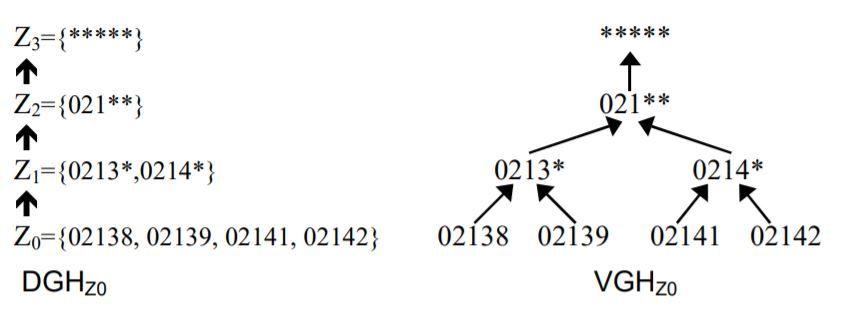
\includegraphics[scale=0.65]{DGH1}
	\caption{DGH dan VGH pada atribut ZIP}
	\label{fig:DGH1}
\end{figure}

\begin{figure}[H]
	\centering
	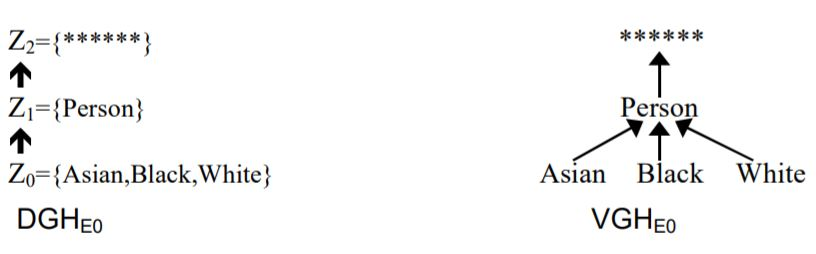
\includegraphics[scale=0.65]{DGH2}
	\caption{DGH dan VGH pada atribut Race}
	\label{fig:DGH2}
\end{figure}

\newpage
\section{K-Anonymity}
\textit{K-anonymity} merupakan model yang paling efektif untuk melindungi privasi saat melakukan publikasi data. \textit{K-anonymity} adalah contoh pemodelan dari keamanan informasi yang bertujuan agar sebuah data tidak dapat dibedakan setidaknya dengan k-1 data lainnya. Dengan kata lain, penyerang tidak dapat mengidentifikasi identitas dari satu data karena k-1 data yang lain memiliki sifat yang sama. Dalam pemodelan k-anonymity, nilai k dapat digunakan sebagai tingkat keamanan privasi. Semakin tinggi nilai k, semakin sulit untuk mengindentifikasi sebuah data. Secara teori, probabilitas identifikasi sebuah data adalah 1 / k. Namun, meningkatkan nilai k juga berpengaruh terhadap nilai informasi yang diperoleh dari sekumpulan data.

\par \textit{K-anonymity} pertama kali diusulkan pada tahun 1998 oleh Sweeney et al. \textit{K-anonymity} tergantung pada menganonimkan kumpulan data asli untuk memenuhi persyaratan anonimisasi, yang dapat digunakan untuk penerbitan data. Teknik anonimisasi yang umum adalah generalisasi dan disembunyikan. Gagasan dasar \textit{K-anonymity} adalah menganonimkan data penerbitan untuk memenuhi persyaratan bahwa setidaknya k buah record yang tidak dapat dibedakan satu sama lain. Yaitu, untuk masing-masing tuple terdapat setidaknya k data dengan nilai yang sama dari quasi-identifiers. Para peneliti telah membuktikan bahwa kompleksitas \textit{k-anonymity} adalah \textit{NP-hard}. \textit{NP-hard} adalah istilah yang sering digunakan untuk menyatakan kompleksitas sebuah algoritma sangat tinggi (eksponensial).

\par Penelitian menunjukkan bahwa sebagian besar pemodelan \textit{k-anonymity} menggunakan metode generalisasi dan supresi. Pendekatan tersebut menderita kehilangan informasi yang signifikan karena mereka sangat bergantung terhadap hubungan relasi antar atribut. Oleh karena itu, hasil anonimisasi menghasilkan nilai kehilangan informasi yang cukup tinggi. Selain itu, algoritma anonimisasi yang ada hanya berfokus pada perlindungan informasi pribadi dan mengabaikan utilitas data yang sebenarnya. Akibatnya, nilai utilitas pada data yang telah dianonimisasi memiliki bernilai rendah. Beberapa algoritma telah dicoba untuk mengimplementasikan pemodelan \textit{k-anonymity}.

\par Algoritma \textit{k-means clustering} akan melakukan beberapa iterasi sampai \textit{centroid} dari semua data tidak lagi berubah atau perubahannya kecil. Algoritma \textit{k-means clustering} tidak mampu untuk menyelesaikan masalah pada atribut yang bernilai kategorikal. Kelebihan dari algoritma \textit{k-means clustering} adalah memiliki hasil pengelompokan yang sudah baik. Kekurangan dari algoritma \textit{k-means clustering} adalah pemilihan centroid awal k-means secara acak, sehingga setelah digeneralisasi hasil pengelompokannya mengakibatkan hilangnya informasi yang besar.

\par Algoritma \textit{k-member} dapat melakukan generalisasi atribut kategorikal dengan memperoleh kualitas informasi yang lebih baik daripada algoritma \textit{k-means clustering}. Namun algoritma \textit{k-member} masih memiliki masalah ketika melakukan pengelompokan data. Kekurangan dari algoritma \textit{k-member} adalah hanya mempertimbangkan pengelompokan terakhir tanpa memperhatikan pengelompokan yang dihasilkan pada proses sebelumnya sehingga menyebabkan distribusi kelompok pada beberapa bagian menjadi kurang tepat. 

\par Untuk menghindari kekurangan pada algoritma \textit{k-means} dan algoritma \textit{k-member} maka kedua konsep ini perlu digabung menjadi sebuah algoritma baru dengan nama algoritma \textit{Greedy k-member clustering}. Algoritma \textit{Greedy k-member clustering} mendapatkan hasil pengelompokan yang lebih tepat dan memiliki nilai informasi yang lebih baik meskipun dilakukan generalisasi. Menggunakan algoritma \textit{Greedy k-member clustering}, pengelompokan data dapat dilakukan satu kali sehingga dapat menurunkan kompleksitas algoritma dan hasil  pemilihan centroid dapat dioptimalkan sehingga hasil pengelompokan dapat ditingkatkan secara signifikan. Hasil akhir dari algoritma \textit{Greedy k-member clustering} adalah data-data yang sejenis sudah dikelompokan pada kelompok data yang sama. Untuk melakukan anonimisasi pada pemodelan \textit{k-anonymity}, digunakan konsep \textit{Hierarchy Based Generalization}. Konsep ini menyamarkan data yang  memiliki nilai quasi-identifier yang sama. Beberapa pemodelan yang dapat digunakan adalah \textit{Domain Generalization Hierarchy}(DGH) dan \textit{Value Generalization Hierarychy} (VGH). Pemodelan VGH akan diterapkan pada data yang nilainya sama dengan data lain dalam satu kelompok. 


\section{Greedy K-Member Clustering}
\label{sec:greedyclustering}
Penelitian menunjukkan bahwa sebagian besar metode \textit{k-anonymity} didasarkan pada generalisasi dan teknik penekanan sehingga menderita dari kehilangan informasi yang signifikan. Masalah pengelompokan dapat meminimalkan kehilangan informasi melalui algoritma \textit{k-member clustering}. Akan tetapi algoritma \textit{k-member clustering} berpotensi memiliki kompleksitas yang eksponensial. Untuk menurunkan kompleksitas tersebut, maka permasalahan algoritma \textit{k-member clustering} dapat didefinisikan sebagai permasalahan algoritma \textit{Greedy}. Algoritma \textit{Greedy k-Member clustering} bertujuan untuk membagi seluruh tuple pada dataset ke masing-masing \textit{cluster} dengan kompleksitas yang lebih baik dan mendukung informasi yang lebih banyak dibandingkan algoritma \textit{clustering} yang lain.

\begin{theorem}
Masalah pengambilan keputusan pada \textit{k-member clustering} adalah \textit{NP-Hard}, artinya memiliki kompleksitas yang eksponensial.
\end{theorem}

\begin{proof}
Melalui pengamatan Aggarwal et al, permasalahan \textit{k-member clustering} dapat diselesaikan dengan kompleksitas polinomial.
\end{proof}

\begin{theorem}
N adalah total data dan k adalah parameter untuk anonimisasi. Setiap \textit{cluster} yang ditemukan oleh algoritma \textit{Greedy k-member clustering} memiliki jumlah tuple minimal sebanyak k, dan jumlah tuple tidak melebihi $2k - 1$.
\end{theorem}

\begin{proof}
S adalah himpunan data. Algoritma ini menemukan \textit{cluster} selama jumlah data yang tersisa sama dengan atau lebih besar dari k, setiap \textit{cluster} berisi k data. Jika total data pada S kurang dari k, maka sisa data akan dikelompokan pada  \textit{cluster} yang sudah ada. Oleh karena itu, ukuran maksimum sebuah \textit{cluster} adalah $2k - 1$.
\end{proof}

\begin{theorem}
N adalah jumlah data dan k menjadi parameter anonimisasi yang ditentukan. Jika $n > k$, kompleksitas algoritma \textit{Greedy k-member clustering} adalah $O(n^2)$.
\end{theorem}

\begin{proof}
Algoritma \textit{Greedy k-member clustering} menghabiskan sebagian besar waktunya untuk memilih data dari S satu per satu hingga mencapai $|S| = k$. Karena ukuran set input berkurang satu pada setiap iterasi, total waktu eksekusi adalah O $(n^2)$.
\end{proof}

\noindent Beberapa hal penting terkait algoritma \textit{Greedy k-means clustering}:

\begin{itemize}
\item Menetapkan tabel S  
\item Menetapkan nilai k
\item Menetapkan jumlah cluster (m) yang ingin dibuat
\begin{align}
m = \left \lfloor \frac{n}{k} \right \rfloor - 1
\end{align}
\end{itemize}


\noindent Berikut adalah langkah kerja algoritma \textit{Greedy k-means clustering} secara lengkap:

\begin{enumerate}
\item Melakukan inisialisasi variabel result dengan himpunan kosong dan variabel r dengan memilih data secara acak dari tabel S

\item Pada kondisi $|S| \geq k$, lakukan perulangan sebagai berikut:

\begin{enumerate}
\item Memilih data baru pada variabel r berdasarkan perbedaaan distance tertinggi dari nilai r sebelumnya. Perbedaan distance dapat dicari menggunakan rumus berikut:
\begin{align*}
\Delta (r_1,r_2) = \sum_{i=1}^{m} \delta_N(r_1[N_i],r_2	[N_i]) +  \sum_{j=1}^{n} \delta_C(r_1[C_j],r_2[C_j])
\end{align*}

\noindent Berikut adalah rumus menghitung distance antar data numerik:
\begin{align*}
\delta_n(v_1,v_2) = \frac{|v_1 - v_2|}{|D|} 
\end{align*}

\vspace{0.4cm}

\noindent Berikut adalah rumus menghitung distance antar data kategorikal:

\begin{align*}
\delta_C(v_1,v_2) = \frac{H(\Lambda(v_i,v_j))}{H(T_D)} 
\end{align*}

\vspace{0.4cm}

\item Membuang himpunan data variabel r pada variabel S

\item Mengisi data dari variabel r pada variabel c.

\item Pada kondisi $|c| \geq k$, lakukan perulangan sebagai berikut:

\begin{enumerate}
\item Memilih data baru terbaik untuk variabel r berdasarkan nilai \textit{Information Loss} (IL) yang paling rendah. \textit{Information Loss} (IL) dapat dicari menggunakan rumus berikut:

\begin{align*}
IL(e)&= |e| \cdot D(e) \\
D(e) &= \sum_{i=1}^{m} \frac{(MAX_{N_i} - MIN_{N_i})}{|N_i|} + \sum_{j=1}^{n}\frac{H(\Lambda(\cup_{C_j}))}{H(T_{C_j})}
\end{align*}

\item Membuang himpunan data dari variabel r pada variabel S

\item Menambahkan himpunan data dari variabel r pada variabel c.

\item Menambahkan himpunan data dari variabel c pada variabel result

\end{enumerate}

\end{enumerate}

\item Pada kondisi $|S| \neq  0$, artinya jika masih terdapat data yang belum dimasukkan pada sebuah \textit{cluster} dari tabel S, lakukan perulangan sebagai berikut:

\begin{enumerate}
\item Memilih data secara acak dari tabel S untuk disimpan pada variabel r

\item Membuang himpunan data dari variabel r pada variabel S

\item Memilih \textit{cluster} terbaik untuk variabel c berdasarkan nilai \textit{Information Loss} (IL) yang paling rendah. \textit{Information Loss} (IL) dapat dicari menggunakan rumus berikut:

\begin{align*}
IL(e)&= |e| \cdot D(e) \\
D(e) &= \sum_{i=1}^{m} \frac{(MAX_{N_i} - MIN_{N_i})}{|N_i|} + \sum_{j=1}^{n}\frac{H(\Lambda(\cup_{C_j}))}{H(T_{C_j})}
\end{align*}

\item Menambahkan himpunan data dari variabel r pada variabel c.

\end{enumerate}

\item Algoritma ini mengembalikan himpunan data berdasarkan jenis \textit{cluster} yang berbeda-beda melalui variabel \textit{result}.

\end{enumerate}

\newpage
\noindent Berikut adalah pseudocode secara lengkap dari algoritma \textit{Greedy k-member clustering}:

\begin{algorithm}[H]
  \caption{Find Best Record}\label{alg:1}
  \begin{algorithmic}[1]
  %-------------- Input & Output -----------------
  \State \textbf{Function} \texttt{find\_best\_record(S,c)}
  \State \textbf{Input:} a set of records S and a cluster c.
  \State \textbf{Output:} a record r $\in$ S such that $IL(c \cup \{r\})$ is minimal
  \\
  %-------------- Baris 1-3 -----------------
  \State{$n = |S|$}
  \State{$min = \infty$}
  \State{$best = null$}
  \For{$i = 1 \ldots n$}
  \State{r = i-th record in S}
  \State{diff = $IL(c \cup \{r\}) - IL(c)$}
  \If{diff < min}
  \State{min = diff}
  \State{best = r}
  \EndIf
  \EndFor
  \State{return best}
  \end{algorithmic}
\end{algorithm}
Algoritma \ref{alg:1} menerima input himpunan data dataset dan sebuah data dengan nilai distance tertinggi dari data terpilih acak. Algoritma ini menghitung selisih \textit{distance} dari dua jenis data yang berbeda. Variabel \textit{diff} pada algoritma ini adalah perbedaan \textit{distance}, dicari dengan penjumlahan \textit{information loss} pada sebuah \textit{cluster} dengan \textit{information loss} pada data ke-i, lalu hasil penjumlahan tersebut dikurangi dengan \textit{information loss} dari \textit{kluster}. Output algoritma ini adalah sebuah data dengan nilai terbaik, yaitu data ke-i dari dataset S dengan nilai \textit{distance} paling kecil.
\begin{algorithm}[H]
  \caption{Find Best Cluster}\label{alg:2}
  \begin{algorithmic}[1]
  %-------------- Input & Output -----------------
  \State \textbf{Function} \texttt{find\_best\_cluster(C,r)}
  \State \textbf{Input:} a set of cluster C and a record r.
  \State \textbf{Output:} a cluster c $\in$ C such that $IL(c \cup \{r\})$ is minimal
  \\
  %-------------- Baris 1-3 -----------------
  \State{$n = |C|$}
  \State{$min = \infty$}
  \State{$best = null$}
  \For{$i = 1 \ldots n$}
  \State{c = i-th cluster in C}
  \State{diff = $IL(c \cup \{r\}) - IL(c)$}
  \If{diff < min}
  \State{min = diff}
  \State{best = c}
  \EndIf
  \EndFor
  \State{return best}
  \end{algorithmic}
\end{algorithm}

Algoritma \ref{alg:2} menerima input himpunan data \textit{cluster} dan sebuah data dengan nilai \textit{distance} tertinggi dari data terpilih acak. Algoritma ini menghitung selisih distance dari dua jenis data yang berbeda. Variabel \textit{diff} pada algoritma ini adalah perbedaan distance, dicari dengan penjumlahan \textit{information loss} pada sebuah \textit{cluster} dengan \textit{information loss} pada data ke-i, lalu hasil penjumlahan tersebut dikurangi dengan \textit{information loss} dari {cluster}. Output algoritma ini adalah data dengan nilai \textit{cluster} terbaik, yaitu data ke-i dari dataset S dengan nilai \textit{distance} paling kecil.

\begin{algorithm}[H]
  \caption{Greedy K-Member Clustering}		 \label{alg:3}
  \begin{algorithmic}[1]
  %-------------- Input & Output -----------------
  \State \textbf{Function} \texttt{greedy\_k\_member\_clustering(S,k)}
  \State \textbf{Input:} a set of records S and a threshold value k
  \State \textbf{Output:} a set of clusters each of which contains at least k records.
  \\
  %-------------- Baris 1-3 -----------------
  \If{$S \leq k$} 
  \State{return S}
  \EndIf
  \\
  \State{$result = \phi$}
  \State{r = a randomly picked record from S}
  \While{$|S| \geq k$}
  \State{r = the furthest record from r}
  \State{S = S - \{r\}}
  \State{c = \{r\}}
  	\While{$|c| < k$}
	\State{r = find\_best\_record(S,c)}  
	\State{S = S - \{r\}}
  	\State{c = c $\cup$ \{r\}}
  	\EndWhile
  	\State{result = result $\cup$ \{c\}}
  \EndWhile
  \While{$S \neq 0$}
  \State{r = a randomly picked record from S}
  \State{S = S - \{r\}}
  \State{c = find\_best\_cluster(result,r)}
  \State{c = c $\cup$ \{r\}}
  \EndWhile
  \State{return result}
  \end{algorithmic}
\end{algorithm}

Algoritma \ref{alg:3} menerima input himpunan data S dan nilai k. Algoritma ini mengeksekusi dua jenis fungsi yang berbeda yaitu fungsi \textit{find\_best\_cluster} untuk mencari \textit{cluster} dengan \textit{distance} terkecil dan fungsi \textit{find\_best\_record} untuk mencari data dengan \textit{distance} terkecil. Output dari algoritma ini adalah himpunan data dari berbagai jenis \textit{cluster} dengan nilai \textit{distance} terkecil.



\section{Metrik Distance, Information Loss} 
\label{theory:dist,il,cf}
Konsep PPDM memberikan solusi untuk mengukur tingkat keamanan, fungsionalitas, dan utilitas data menggunakan beberapa jenis metrik.  Beberapa metrik yang umum digunakan pada pengujian kualitas data yang telah dianonimisasi adalah \textit{distance} dan \textit{information loss}. Secara umum, pengukuran metrik dilakukan dengan membandingkan hasil anonimisasi dengan dataset sesungguhnya. 

\subsection{\textit{Distance}} 
\textit{Distance} adalah salah satu perhitungan untuk menyatakan akurasi terhadap utilitas sebuah data. \textit{Distance} merupakan faktor yang paling penting untuk menentukan hasil pengelompokan data. Pemilihan \textit{distance} yang baik dapat mencapai hasil klasifikasi dengan lebih optimal. Perhitungan \textit{distance} dilakukan berdasarkan pengelompokan tipe data numerik atau kategorikal. Karena masalah \textit{k-anonymity} menggunakan atribut numerik dan kategorikal, maka membutuhkan cara khusus untuk mengitung \textit{distance} dari kedua jenis data pada saat yang sama. 

\subsubsection{\textit{Distance} Data Numerik}
\textit{Distance} data numerik direpresentasikan sebagai nilai rentang. Beberapa atribut pada \textit{distance} numerik yaitu |D| adalah jumlah data pada sebuah domain berdasarkan satu atribut numerik, $v_1$, $v_2$ adalah nilai atribut numerik. \textit{Distance} data numerik dihitung menggunakan rumus berikut:

\begin{equation}
\delta_n(v_1,v_2) = \frac{|v_1 - v_2|}{|D|} 
\end{equation}

\subsubsection{Distance Data Kategorikal}
\textit{Distance} data kategorikal direpresentasikan sebagai \textit{taxonomy tree}. Beberapa atribut pada distance kategorikal yaitu |D| adalah jumlah data pada domain kategorikal, TD adalah \textit{taxonomy tree} untuk domain D,  $H(\Lambda(v_i,v_j))$ adalah jarak dari satu \textit{subtree} ke \textit{subtree} lain, $H(T_D)$ adalah tinggi dari \textit{taxonomy tree}. \textit{Distance} data kategorikal dihitung menggunakan rumus berikut:

\begin{equation}
\delta_C(v_1,v_2) = \frac{H(\Lambda(v_i,v_j))}{H(T_D)} 
\end{equation}

\subsubsection{Distance Record}
Beberapa atribut pada \textit{distance record} yaitu $r_1[N_i]$, $r_2[N_i]$ adalah nilai dari atribut numerik, $r_1[C_j]$, $r_2[C_j]$ adalah nilai dari atribut kategorikal, $\delta_N$ adalah \textit{distance} data numerik, $\delta_C$ adalah \textit{distance} data kategorikal. \textit{Distance} record dihitung menggunakan rumus berikut:
\begin{align}
\Delta (r_1,r_2) = \sum_{i=1}^{m} \delta_N(r_1[N_i],r_2	[N_i]) +  \sum_{j=1}^{n} \delta_C(r_1[C_j],r_2[C_j])
\end{align}


\subsection{Information Loss}
\textit{Information Loss} (IL) digunakan untuk mengevaluasi seberapa baik kinerja algoritma \textit{k-anonymity} terhadap utilitas sebuah data. Dalam menghitung \textit{Information Loss} (IL), perlu mendefinisikan beberapa atribut seperti \textit{cluster} $e = {r_1,\ldots,r_k}$  untuk \textit{quasi-identifier} yang terdiri dari atribut numerik ${N1,\ldots, Nm}$ dan atribut kategorikal ${C_1,\ldots,C_n}$, $T_{C_i}$ adalah \textit{taxonomy tree} untuk domain kategorikal $C_i$, $MIN_{N_i}$ dan $MAX_{N_i}$ adalah nilai minimum dan maksimum pada cluster $e$ untuk atribut Ni, $\cup_{C_i}$ adalah sekumpulan nilai pada \textit{cluster} $e$ berdasarkan atribut $C_i$. \\

\noindent \textit{Information loss} dihitung dengan rumus sebagai berikut:
\begin{align}
IL(e)&= |e| \cdot D(e) \\
D(e) &= \sum_{i=1}^{m} \frac{(MAX_{N_i} - MIN_{N_i})}{|N_i|} + \sum_{j=1}^{n}\frac{H(\Lambda(\cup_{C_j}))}{H(T_{C_j})}
\end{align}

\noindent Total \textit{Information Loss} dihitung dengan rumus sebagai berikut:
\begin{align}
Total-IL(AT) = \sum_{e \in \varepsilon}^{}  IL(e)
\end{align}

\noindent Semakin besar total \textit{information loss} yang dihasilkan maka informasi yang dihasilkan semakin kurang akurat. Oleh karena itu perlu dilakukan beberapa eksperimen terhadap penentuan nilai k pada algoritma \textit{Greedy k-member clustering} agar dihasilkan total \textit{information loss} seminimal mungkin sehingga hasil \textit{clustering} dan klasifikasi dengan nilai akurasi yang tinggi.

\newpage
\section{Sistem Terdistribusi}
Sistem terdistribusi adalah kumpulan komputer berjalan secara independen, yang saling terhubung dan saling bekerja sama untuk mencapai satu tujuan yang sama. Konsep penting terkait sistem terdistribusi adalah setiap komputer bekerja untuk satu tujuan yang sama, setiap komputer mengerjakan tugas yang berbeda dengan komputer lainnya, pembagian jumlah tugas dilakukan secara adil, setiap komputer memiliki jalur komunikasi yang sama untuk saling bertukar informasi.

\subsection{Manfaat Sistem Terdistribusi}
Permasalahan sistem terdistribusi bukan difokuskan terhadap penggunaan sistem terdistribusi, melainkan alasan yang tepat untuk menggunakan sistem terdistribusi. Sistem terdistribusi dibutuhkan karena adanya peningkatan skala dalam pengolahan data dan munculnya sistem yang lebih handal untuk melakukan pemrosesan data. 
\\\\
Berikut adalah beberapa manfaat penggunaan sistem terdistribusi bagi efektivitas pengolahan big data:

\begin{itemize}
\item \textit{Horizontal Scalability}\\
Sistem terdistribusi menawarkan kemampuan untuk melakukan pemrosesan komputasi skala besar pada big data dengan harga yang murah.

\item \textit{Reliability}\\
Sistem terdistribusi dapat diandalkan karena proses komputasi pada sistem terdistribusi bergantung pada banyaknya komputer yang saling berkomunikasi satu sama lain untuk mencapai tujuan yang sama.
 
\item \textit{Performance}\\
Sistem terdistribusi dapat menangani proses komputasi tugas secara efisien karena beban kerja sesungguhnya dibagi menjadi beberapa bagian dan tersebar di beberapa komputer. 
\end{itemize}

\subsection{Tantangan Sistem Terdistribusi} 
Tantangan penggunaan sistem terdistribusi adalah pemrosesan data skala besar dengan handal. Dalam perancangan sistem terdistribusi, sering ditemui kesulitan pada pemecahan masalah untuk kasus-kasus tertentu. 
\\\\
Berikut adalah tiga tantangan paling umum ditemui ketika melakukan implementasi program pada sistem terdistribusi:

\begin{itemize}
\item Penjadwalan\\
Kekuatan komputasi ada batasnya, sehingga sistem terdistribusi harus dapat memutuskan pekerjaan mana yang harus dikerjakan lebih dulu.
\item Latensi\\
Dengan pertukaran data antara perangkat keras dan perangkat lunak menggunakan jalur komunikasi jaringan, sehingga nilai latensi menjadi sangat tinggi. 
\item Observasi\\
Ketika sistem terdistribusi menjadi kompleks, kemampuan pengamatan untuk memahami kegagalan pada sistem terdistribusi merupakan tantangan besar komputer. 
\end{itemize}

\newpage
\section{Big Data}
\textit{Big data} adalah data yang besar dan kompleks sehingga tidak mungkin sistem tradisional dapat memproses dan bekerja pada lingkungan data yang besar secara maksimal. Data dapat dikategorikan sebagai data besar berdasarkan berbagai faktor. Konsep utama yang umum dalam semua faktor  adalah jumlah data. Berikut adalah karakteristik 5V untuk \textit{big data}:

\begin{itemize}
\item \textit{Volume}\\
\textit{Volume} mengacu pada jumlah data yang sangat besar. Data tumbuh begitu besar sehingga sistem komputasi tradisional tidak lagi dapat menanganinya seperti yang kita inginkan.

\item \textit{Velocity}\\
\textit{Velocity} mengacu pada kecepatan di mana data dihasilkan. Setiap hari, sejumlah besar data dihasilkan, disimpan, dan dianalisis. Data dihasilkan dengan kecepatan kilat di seluruh dunia. Teknologi \textit{big data} memungkinkan untuk mengeksplorasi data, saat data itu dihasilkan.

\item \textit{Variety}\\
\textit{Variety} mengacu pada berbagai jenis data. Data terutama dikategorikan ke dalam data terstruktur dan tidak terstruktur. Faktanya, lebih dari 75 persen data dunia ada dalam bentuk yang tidak terstruktur. 

\item \textit{Veracity}\\
\textit{Veracity} mengacu pada kualitas data. Ketika menyimpan beberapa data yang besar, apabila tidak ada gunanya di masa depan, maka membuang-buang sumber daya untuk menyimpan data tersebut. Jadi, kita harus memeriksa kepercayaan data sebelum menyimpannya. 

\item \textit{Value}\\
\textit{Value} adalah bagian terpenting dari big data. Organisasi menggunakan data besar untuk menemukan nilai informasi baru. Menyimpan sejumlah besar data sampai pada ekstraksi informasi yang bermakna dari sekumpulan data tersebut.
\end{itemize}

\section{Analisis Big Data}
\noindent Analisis \textit{big data} adalah proses menggunakan algoritma analisis yang berjalan pada \textit{platform} pendukung yang kuat untuk mengungkap potensi yang disembunyikan dalam data besar, seperti pola tersembunyi atau korelasi yang tidak diketahui. Analisis \textit{big data} dapat dikategorikan ke dalam dua jenis pemrosesan. Berikut adalah jenis analisis pada \textit{big data}:

\begin{itemize}
\item 
\textit{Batch Processing}\\
\textit{Batch processing} adalah sekumpulan data disimpan terlebih dahulu, lalu pada waktu tertentu data yang telah terkumpul akan dilakukan analisis. \textit{MapReduce} telah menjadi model penerapan batch processing pada umumnya. Ide dari \textit{MapReduce} adalah data yang besar dibagi menjadi potongan data yang lebih kecil. Selanjutnya, potongan-potongan data ini diproses secara paralel dan secara terdistribusi untuk dianalisis lebih lanjut. 

\item
\textit{Streaming Processing}\\
\textit{Streaming processing} mengasumsikan nilai informasi data yang diperoleh bergantung kepada seberapa cepat data dapat diolah secara \textit{real time}. Pengertian dari \textit{real time} adalah data diolah secara langsung ketika data tersebut diperoleh. Dalam paradigma ini, data diambil melalui aliran data. Karena aliran data yang masuk sangat cepat dan membawa volume yang cukup besar, maka hanya sebagian kecil data yang dapat disimpan dan diolah dalam memori yang terbatas. Paradigma \textit{streaming processing} biasanya digunakan untuk analisis aplikasi online dalam tingkat satuan detik maupun milidetik.
\end{itemize}

\newpage
\section{Hadoop}
Hadoop adalah \textit{framework} yang memanfaatkan beberapa komputer untuk menyelesaikan masalah yang melibatkan volume data sangat besar. Pada Gambar \ref{fig:hadoop_intro}, Hadoop memecah input dari pengguna menjadi beberapa blok data dan masing-masing blok data diproses menggunakan konsep \textit{MapReduce} di mana data akan diproses secara paralel pada sistem terdistribusi. Hadoop adalah \textit{framework} yang dibangun dengan bahasa Java. Hadoop bekerja dari satu komputer utama ke ribuan komputer dengan melakukan perhitungan dan penyimpanan lokal pada setiap komputer. 

\begin{figure}[H]
	\centering
	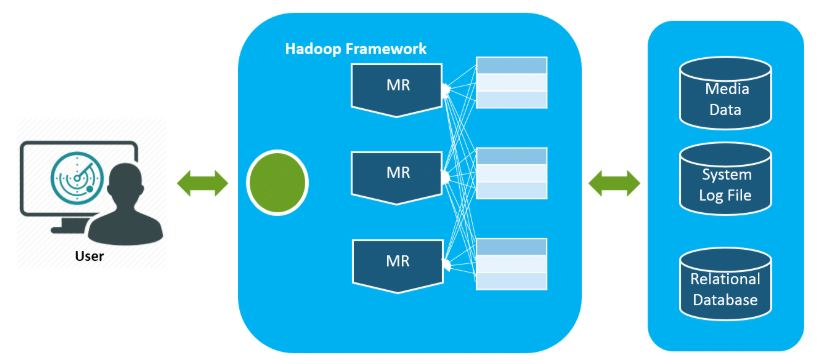
\includegraphics[scale=0.62]{hadoop_intro}
	\caption{Gambaran Umum Cara Kerja Hadoop}
	\label{fig:hadoop_intro}
\end{figure}

\noindent Hadoop memiliki karakteristik sebagai berikut:
\begin{itemize}
\item Hadoop menyediakan penyimpanan HDFS dan menggunakan pemodelan \textit{MapReduce}.
\item Hadoop melakukan replikasi data sejenis pada beberapa komponen berbeda. 
\item Hadoop fleksibel terhadap pengaturan jumlah komponen yang bekerja.
\item Hadoop dioptimalkan untuk bekerja pada lingkungan \textit{big data}.
\item Hadoop menulis data sekali dan membaca data berulang kali.

\end{itemize}

\subsection{Ekosistem Hadoop}
\begin{figure}[H]
	\centering
	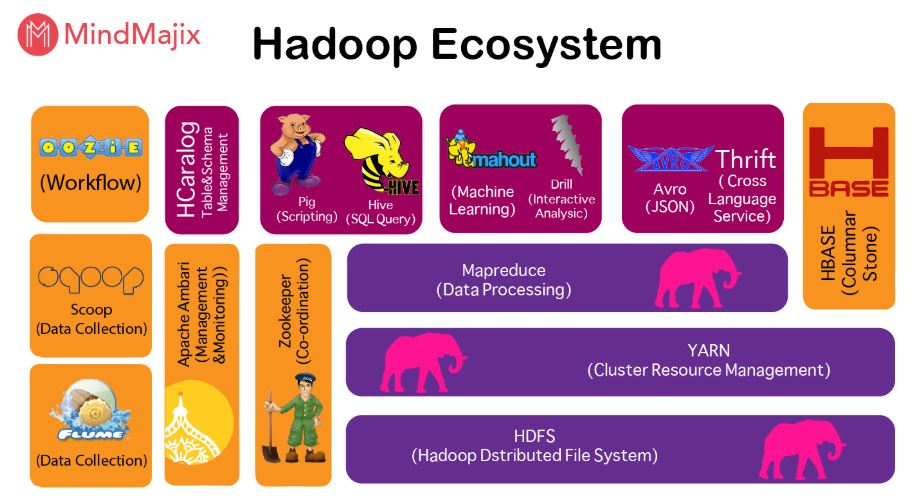
\includegraphics[scale=0.65]{hadoop_ecosystem}
	\caption{Ekosistem Hadoop}
	\label{fig:hadoop_ecosystem}
\end{figure}
Gambar \ref{fig:hadoop_ecosystem} menunjukan bahwa Hadoop dapat bekerja secara bersamaan dengan teknologi \textit{big data} lainnya seperti Spark, HBase, Cassandra, STORM, dan lain-lain untuk memenuhi berbagai macam kebutuhan dalam pengolahan dan analisis pada \textit{big data}.

\subsection{Arsitektur Hadoop}
\begin{figure}[H]
	\centering
	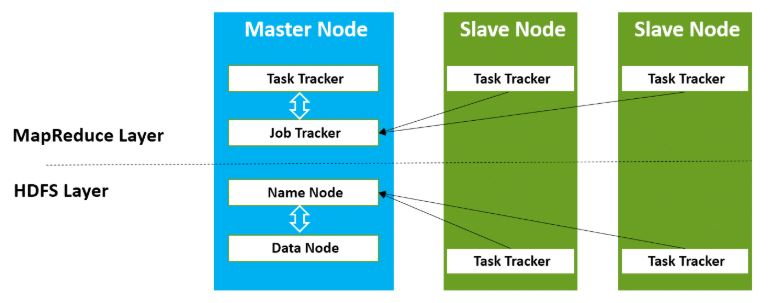
\includegraphics[scale=0.85]{arsitektur_hadoop}
	\caption{Arsitektur Hadoop}
	\label{fig:arsitektur_hadoop}
\end{figure}
Gambar \ref{fig:arsitektur_hadoop} menunjukan arsitektur Hadoop yang tersusun atas \textit{MapReduce} dan \textit{Hadoop Distributed File System} (HDFS). Masing-masing bagian memiliki dua jenis node yaitu \textit{master node} dan \textit{slave node}. \textit{Master node} mengatur jumlah pekerjaan yang diberikan kepada dirinya sendiri dan \textit{slave node}. \textit{Slave node} mengerjakan pekerjaan yang diberikan oleh \textit{master node}.


\subsection{HDFS}
HDFS adalah sistem \textit{file} terdistribusi pada Hadoop dengan menyediakan penyimpanan data yang handal, mendukung partisi, dan toleran terhadap kesalahan pada hardware. HDFS bekerja erat dengan MapReduce dengan mendistribusikan penyimpanan dan perhitungan di seluruh \textit{cluster} dengan menggabungkan sumber daya penyimpanan yang dapat dipartisi tergantung kebutuhan. 
\\\\
HDFS terdiri dari beberapa komponen, yaitu:

\begin{itemize}
\item \textit{NameNode}\\
\textit{NameNode} adalah sebuah komputer yang bertindak sebagai \textit{master node}, sedangkan. \textit{NameNode} bertanggungjawab menyimpan informasi tentang penempatan blok-blok data dalam \textit{Hadoop cluster}. Ia bertanggungjawab mengorganisir dan mengontrol blok-blok data yang disimpan tersebar dalam komputer-komputer yang menyusun \textit{Hadoop cluster}. 

\item \textit{DataNode}\\
\textit{DataNode} adalah elemen penyimpanan utama HDFS yang menyimpan blok data dan permintaan baca / tulis layanan pada \textit{file} yang disimpan di HDFS. \textit{DataNode} dikendalikan oleh \textit{NameNode}. Blok yang disimpan dalam \textit{DataNode} direplikasi sesuai konfigurasi untuk memberikan keandalan dan ketersediaan tinggi. Blok yang direplikasi ini didistribusikan di seluruh cluster untuk memberikan perhitungan yang cepat.
\end{itemize}

\subsection{MapReduce}
\textit{MapReduce} adalah kerangka kerja pemrograman untuk komputasi terdistribusi yang dibuat oleh Google menggunakan membagi dan menaklukkan metode untuk memecah masalah data besar yang kompleks menjadi unit-unit kecil pekerjaan dan memprosesnya sejajar. Pemodelan \textit{MapReduce} terdiri dari dua fungsi, yaitu \textit{Mapper} dan \textit{Reducer}. 

\begin{figure}[H]
	\centering
	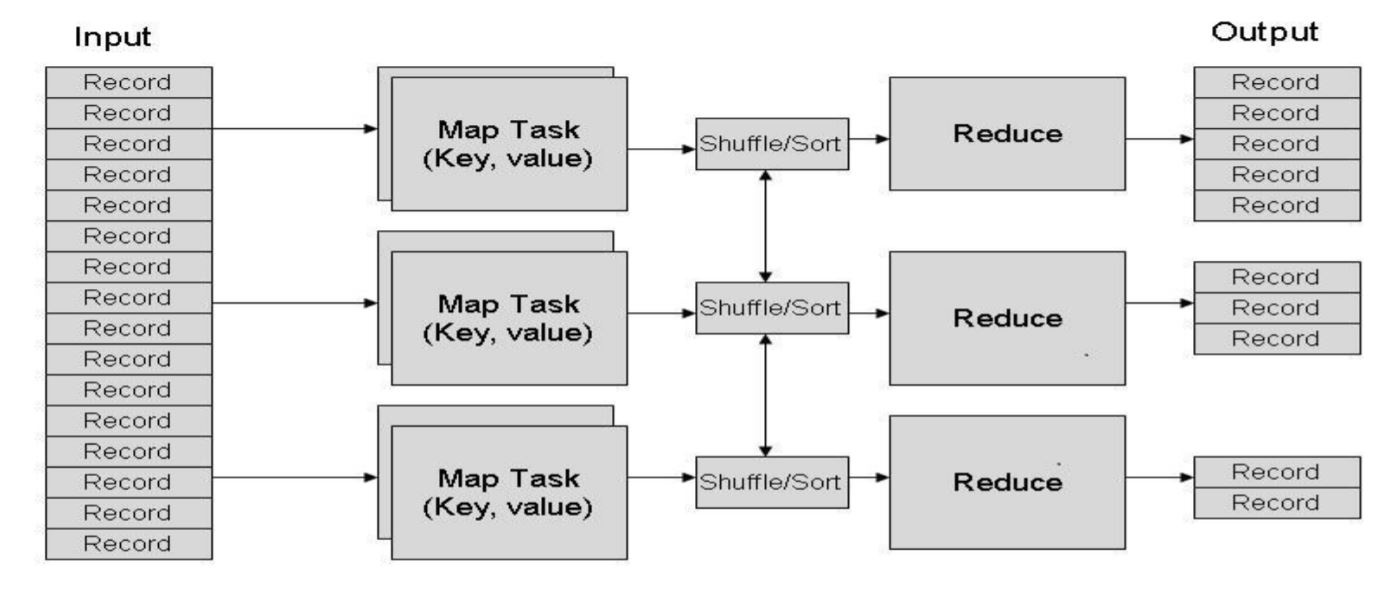
\includegraphics[scale=0.5]{MapReduceImage}
	\caption{Tahapan pada MapReduce}
	\label{fig:MapReduceImage}
\end{figure}

\noindent Pada Gambar \ref{fig:MapReduceImage}, tahapan \textit{MapReduce} dapat dibagi menjadi dua fungsi utama:

\begin{itemize}
\item \textit{Mapper}\\
Tugas fungsi \textit{Mapper} adalah memetakan blok data kedalam pasangan <\textit{key},\textit{value}>. \textit{Key,value} pada \textit{Mapper} tidak harus memiliki tipe data yang sama satu sama lain. Pasangan <\textit{key},\textit{value}> yang mungkin terjadi pada fungsi \textit{Mapper} adalah tidak memiliki pasangan atau memiliki banyak pasangan.

\item Reducer\\
Reducer memiliki 3 fase utama: \textit{shuffle, sort} dan \textit{reducer}. Berikut adalah penjelasan dari tahapan yang dilakukan oleh fungsi \textit{Reducer}:

\begin{enumerate}
\item Shuffle \\
\textit{Shuffle} adalah fase pada data antara untuk menggabungkan semua nilai menjadi koleksi yang terkait dengan kunci yang sama.
\item \textit{Sort} \\
Pasangan <\textit{key},\textit{value}> pada satu node secara otomatis diurutkan oleh Hadoop sebelum diberikan kepada \textit{reducer}. Penyortiran dilakukan berdasarkan keterurutan nilai \textit{key}. 
\item \textit{Reducer} \\
Hasil \textit{mapper} yang diacak dan diurutkan disediakan untuk \textit{Reducer}. Tahap ini membuat pasangan <\textit{key}, \textit{(list of value)}> baru berdasarkan pengelompokan \textit{key}.
\end{enumerate}

\end{itemize}

\noindent \textit{MapReduce} memiliki beberapa komponen, yaitu:

\begin{itemize}
\item \textit{JobTracker}\\
\textit{JobTracker} berjalan pada master node untuk memonitor tugas-tugas \textit{MapReduce} yang telah dijalankan oleh \textit{TaskTracker} pada node salve. Tugas \textit{JobTracker} adalah mengalokasikan pekerjaan yang sesuai untuk \textit{TaskTracker} tertentu tergantung pada berapa banyak slot tugas yang tersedia. 
\item \textit{TaskTracker}\\
\textit{TaskTracker} berjalan pada masing-masing node \textit{slave}. \textit{TaskTracker} menerima pekerjaan dari \textit{JobTracker} dan menjalankan operasi \textit{MapReduce}. Setiap \textit{TaskTracker} memiliki jumlah slot pekerjaan yang terbatas. \textit{TaskTracker} mengatur pelaksanaan setiap operasi \textit{MapReduce} pada setiap node \textit{slave}. 
\end{itemize}

\newpage
\section{Spark} 
\label{sec:konsep_spark}
Spark adalah teknologi komputasi \textit{cluster} yang dirancang untuk komputasi cepat. Spark adalah paradigma pemrosesan data berukuran besar yang dikembangkan oleh para peneliti University of California di Berkeley. Spark adalah alternatif dari Hadoop MapReduce untuk mengatasi keterbatasan pemrosesan input output yang tidak efisien pada disk, dengan menggunakan memori. Fitur utama Spark adalah melakukan komputasi di dalam memori sehingga waktu komputasi menjadi lebih singkat dibandingkan waktu komputasi di dalam disk.
\\\\
Berikut adalah karakteristik dari Spark:
\begin{itemize}
\item Kecepatan\\
Spark adalah alat komputasi klaster tujuan umum. Ini menjalankan aplikasi hingga 100 kali lebih cepat dalam memori dan 10 kali lebih cepat pada disk daripada Hadoop. Spark mengurangi jumlah operasi baca/tulis pada disk dan menyimpan data dalam memori.


\item Mudah untuk diatur\\	
Spark dapat melakukan pemrosesan batch, analisis data secara interaktif, machine learning, dan streaming data. Semuanya pemrosesan tersebut dikerjakan pada satu komputer yang sama. Fungsi ini menjadikan Apache Spark sebagai mesin analisis data yang lengkap. 


\item Analisis secara real-time\\
Spark dapat dengan mudah memproses data \textit{real-time}, misalnya \textit{streaming} data secara \textit{real-time} untuk ribuan peristiwa/detik. Contoh dari sumber \textit{streaming} data adalah Twitter, Facebook, Instagram. \textit{Streaming} data dapat diproses secara efisien oleh Spark.
\end{itemize}

\subsection{Ekosistem Spark}
\begin{figure}[H]
	\centering
	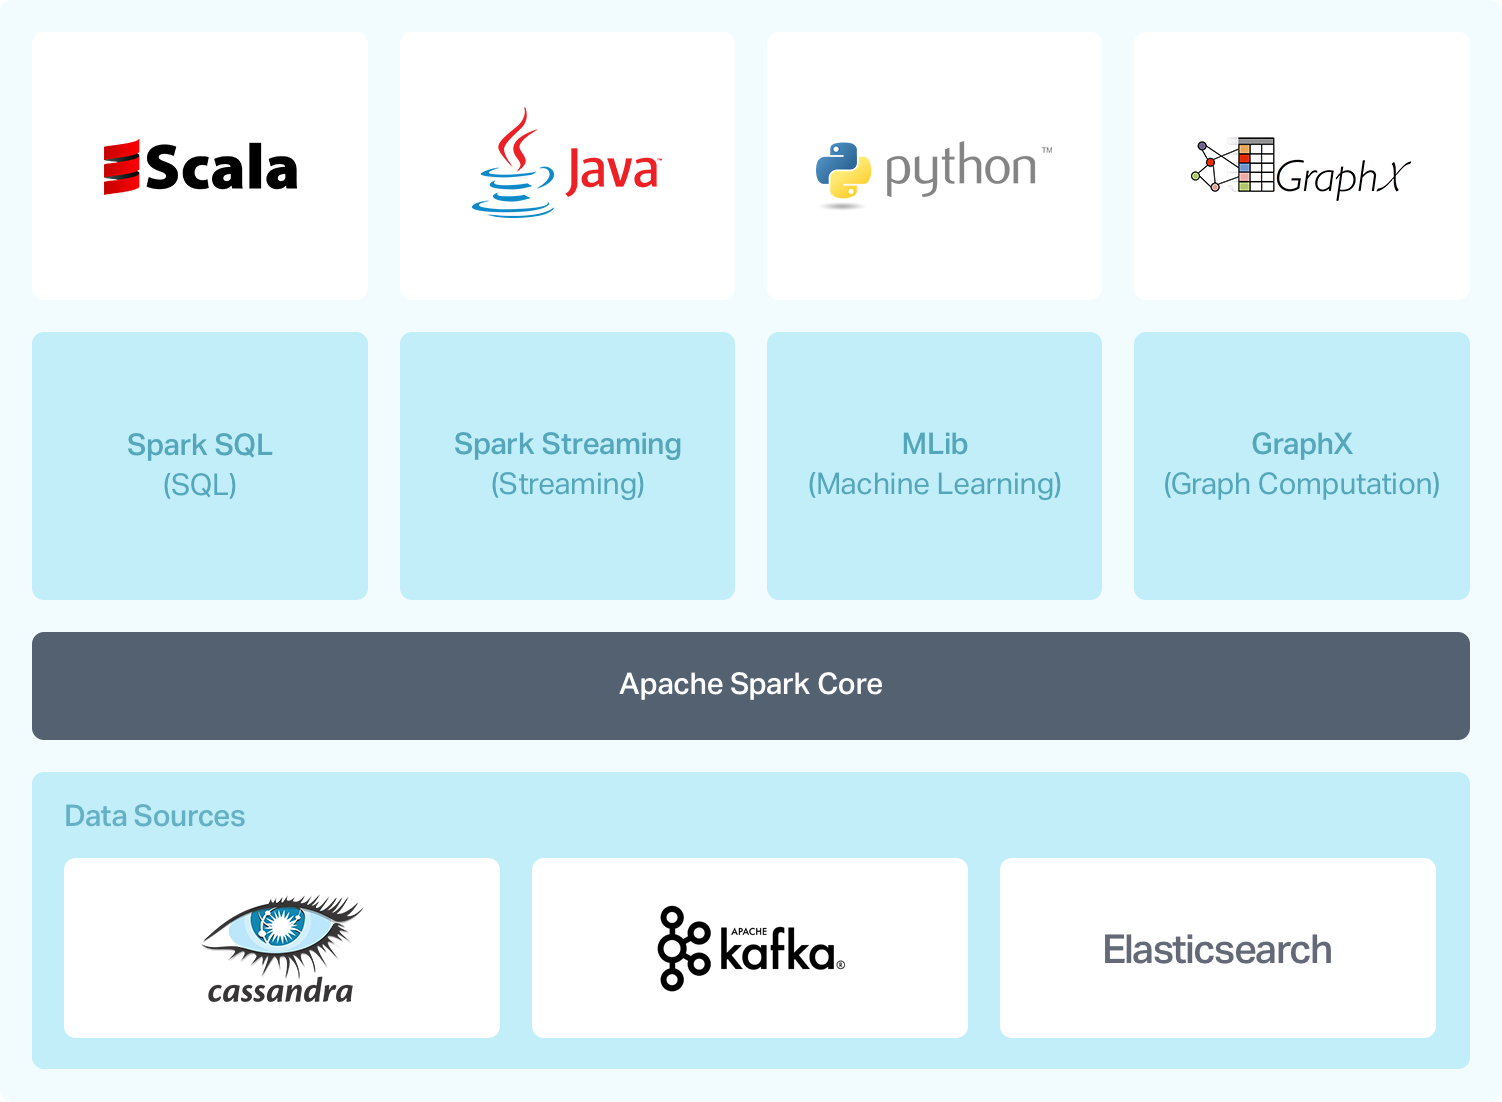
\includegraphics[scale=0.18]{spark_ecosystem}
	\caption{Ekosistem Spark}
	\label{fig:spark_ecosystem}
\end{figure}
Gambar \ref{fig:spark_ecosystem} menunjukan bahwa Spark bekerja sama dengan teknologi \textit{big data} lain untuk memenuhi berbagai macam kebutuhan dalam pengolahan \textit{big data}. Masing-masing warna pada Gambar \ref{fig:spark_ecosystem} mewakili jenis teknologi yang dipakai pada Spark. Spark SQL, Spark Streaming, Spark MLlib adalah library tambahan pada Spark. Cassandra, Kafka, dan ElasticSearch adalah \textit{framework} untuk melakukan pengumpulan data secara \textit{streaming}. Sedangkan scala, java, dan python adalah bahasa pemrograman yang dapat digunakan pada Spark.

\subsection{Arsitektur Spark}
\label{sec:arsitektur_spark}
\begin{figure}[H]
	\centering
	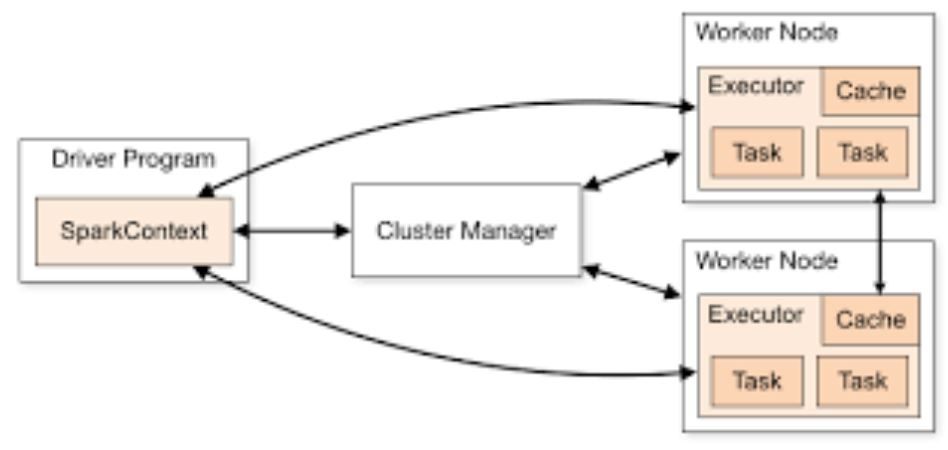
\includegraphics[scale=0.7]{arsitektur_spark2}
	\caption{Arsitektur Spark}
	\label{fig:arsitektur_spark2}
\end{figure}
Berdasarkan Gambar \ref{fig:arsitektur_spark2}, berikut adalah tahapan kerja pada arsitektur Spark:

\begin{enumerate}

\item
\textit{Program Driver} memanggil program utama aplikasi dan membuat \textit{SparkContext} dan \textit{Spark Driver}. \textit{SparkContext} terdiri dari semua fungsi dasar. \textit{Spark Driver} berisi \textit{DAG Scheduler, Task Scheduler, Backend Scheduler}, dan \textit{Block Manager}.

\item
\textit{Spark Driver} dan \textit{SparkContext} secara kolektif mengawasi pelaksanaan pekerjaan di dalam \textit{cluster}. \textit{Spark Driver} bekerja sama dengan \textit{Cluster Manager} untuk membagian pekerjaan ke setiap \textit{Worker Node}. 

\item
\textit{Worker Node} menjalankan tugas yang diberikan oleh \textit{Cluster Manager} dan mengembalikannya ke \textit{SparkContext}. \textit{Worker Node} bertanggung jawab atas pelaksanaan tugas yang diberikan. 

\end{enumerate}


\subsection{Jenis Instalasi pada Spark}
\label{sec:instalasi_spark}
\begin{figure}[H]
	\centering
	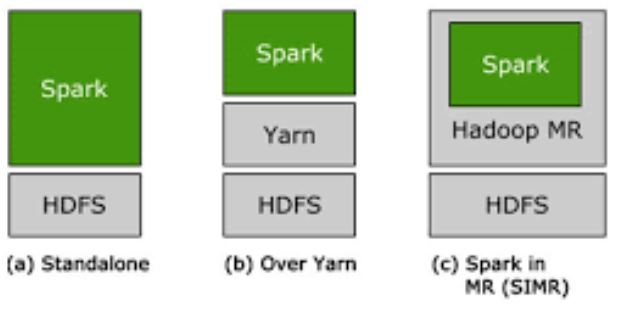
\includegraphics[scale=0.7]{arsitektur_spark}
	\caption{Arsitektur Spark}
	\label{fig:arsitektur_spark}
\end{figure}

Berdasarkan Gambar \ref{fig:arsitektur_spark}, berikut adalah jenis-jenis instalasi pada Spark:

\begin{itemize}
\item \textit{Standalone}\\  
Spark berdiri diatas HDFS Hadoop. Spark memungkinkan untuk mengakses data pada HDFS Hadoop untuk membaca input dan menulis output.

\item \textit{Hadoop Yarn}\\
Spark dapat berjalan pada Hadoop Yarn tanpa memerlukan instalasi atau meminta hak akses root apapun. Hadoop Yarn membantu integrasi Spark pada ekosistem Hadoop.

\item \textit{Spark In MapReduce} (SIMR)\\ 
SIMR digunakan untuk menjalankan pekerjaan Spark secara independen. Jenis instalasi ini sudah tidak lagi berlaku untuk Spark versi 2.0
\end{itemize}

\subsection{Resilient Distibuted Datasets (RDD)}
\label{sec:rdd}
\par RDD adalah kumpulan objek terdistribusi yang disimpan dalam memori atau \textit{disk} pada beberapa \textit{cluster}. Gambar \ref{fig:rdd_intro} menunjukan bahwa RDD tersebar menjadi beberapa partisi sehingga partisi tersebut dapat disimpan dan diproses pada komputer yang berbeda. RDD adalah struktur data yang \textit{immutable}, artinya data tersebut hanya dapat dibaca dan tidak dapat diubah nilainya. RDD dalam Spark dapat di simpan dalam \textit{cache} dan digunakan lagi untuk kebutuhan di masa depan. 

\begin{figure}[H]
	\centering
	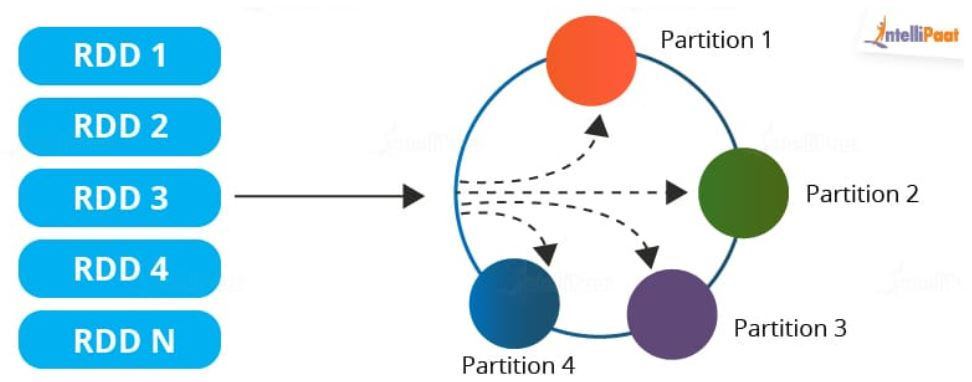
\includegraphics[scale=0.5]{rdd_intro}
	\caption{Cara Kerja RDD}
	\label{fig:rdd_intro}
\end{figure}

\subsubsection{Beberapa Sifat dari RDD}
\noindent Gambar \ref{fig:rdd_feature} menunjukan sifat dari RDD, berikut adalah penjelasannya:
\begin{itemize}
\item \textit{Lazy evaluation}: operasi pada Spark hanya akan dilakukan ketika hasilnya akan dibutuhkan saat itu juga, menggunakan perintah tertentu.

\item \textit{Immutability}: data yang disimpan dalam RDD hanya dapa dibaca dan tidak dapat mengubah nilai data di dalam RDD. 

\item \textit{Fault Tolerance}: RDD melakukan toleransi kesalahan dengan melacak histori data untuk memulihkan data yang hilang secara otomatis jika eksekusi gagal.

\item \textit{In-memory computation}: RDD menyimpan data secara langsung dalam memori (RAM) daripada disk sehingga memberikan akses yang lebih cepat.

\item \textit{Partitioning}: partisi dapat dilakukan pada RDD untuk membagi perkerjaan pada \textit{Worker Node} di beberapa komputer.
\end{itemize}

\begin{figure}[H]
	\centering
	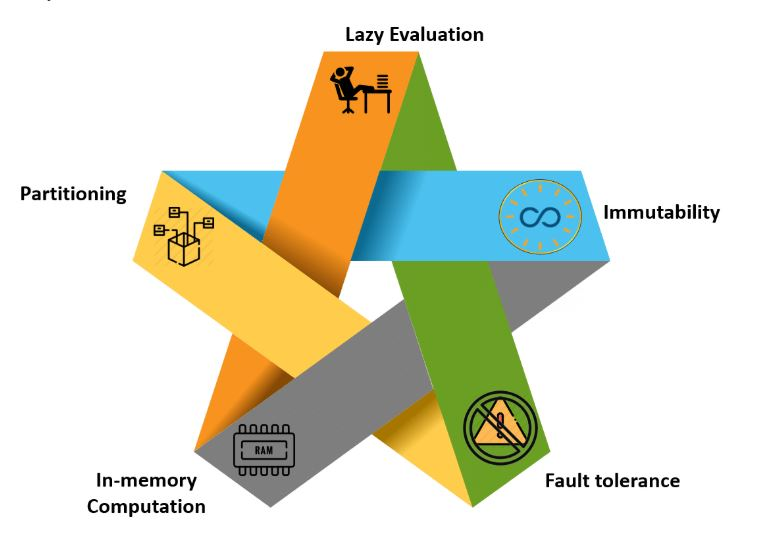
\includegraphics[scale=0.55]{rdd_feature}
	\caption{Fitur pada RDD}
	\label{fig:rdd_feature}
\end{figure}



\subsubsection{Fungsi pada RDD}
\label{sec:fungsi_rdd}
\noindent Berikut adalah penjelasan singkat dan contoh dari jenis operasi pada RDD:

\begin{itemize}
\item Fungsi \textit{Transformation}\\
Fungsi \textit{Tranformation} adalah operasi pada RDD untuk mengembalikan output berupa RDD baru. Fungsi \textit{transformation} pada RDD dilakukan secara \textit{lazy}, sehingga fungsi \textit{tranformation} hanya akan dikerjakan apabila dipanggil pada fungsi \textit{action}. Fungsi \textit{transformation} pada RDD akan dijelaskan pada tabel dibawah ini.\\

\begin{tabular}{|l|p{10cm}|}
\hline 
\rule[-1ex]{0pt}{2.5ex} Fungsi & Deskripsi \\ 
\hline 
\rule[-1ex]{0pt}{2.5ex} map() & Mengembalikan RDD baru dengan menerapkan fungsi pada setiap elemen data \\ 
\hline 
\rule[-1ex]{0pt}{2.5ex} filter() & Mengembalikan RDD baru yang dibentuk dengan memilih elemen-elemen sumber di mana fungsi mengembalikan true \\ 
\hline 
\rule[-1ex]{0pt}{2.5ex} reduceByKey() & Menggabungkan nilai-nilai kunci menggunakan fungsi \\ 
\hline 
\rule[-1ex]{0pt}{2.5ex} groupByKey() & Mengonversi pasangan (kunci, nilai) menjadi pasangan (kunci, <iterable value>) \\ 
\hline 
\rule[-1ex]{0pt}{2.5ex} union() & Mengembalikan RDD baru yang berisi semua elemen dan argumen dari RDD sumber \\ 
\hline 
\rule[-1ex]{0pt}{2.5ex} intersection() & Mengembalikan RDD baru yang berisi persimpangan elemen dalam dataset \\ 
\hline 
\end{tabular} 

\item Fungsi \textit{Action}\\
Fungsi \textit{Action} adalah operasi yang mengembalikan nilai output ke dalam terminal atau melakukan penulisan data pada sistem penyimpanan eksternal. Fungsi \textit{Action} memaksa evaluasi pada RDD yang akan dipanggil, untuk menghasilkan output. Fungsi \textit{Action} pada RDD akan dijelaskan pada tabel dibawah ini.\\

\begin{tabular}{|l|p{10cm}|}
\hline 
\rule[-1ex]{0pt}{2.5ex} Fungsi & Deskripsi \\ 
\hline 
\rule[-1ex]{0pt}{2.5ex} count() & Mendapat jumlah elemen data dalam RDD \\ 
\hline 
\rule[-1ex]{0pt}{2.5ex} collect() & Mendapat semua elemen data dalam RDD sebagai array \\ 
\hline 
\rule[-1ex]{0pt}{2.5ex} reduce() & Agregat elemen data ke dalam RDD dengan mengambil dua argumen dan mengembalikan satu \\ 
\hline 
\rule[-1ex]{0pt}{2.5ex} take(n) & Mengambil n elemen pertama dari RDD \\ 
\hline 
\rule[-1ex]{0pt}{2.5ex} foreach(operation) & Menjalankan operasi untuk setiap elemen data dalam RDD \\ 
\hline 
\rule[-1ex]{0pt}{2.5ex} first() & Mengambil elemen data pertama dari RDD \\ 
\hline 
\end{tabular} 
\end{itemize}

\subsection{DataFrame}
\label{sec:dataframe}
\textit{DataFrame} adalah kumpulan data yang didistribusikan, disusun dalam baris dan kolom. Setiap kolom dalam \textit{DataFrame} memiliki nama dan tipe terkait. \textit{DataFrame} mirip dengan tabel database tradisional, yang terstruktur dan ringkas. \textit{DataFrame} adalah basis data relasional dengan teknik optimisasi yang lebih baik. Dengan menggunakan \textit{DataFrame}, kueri SQL dapat dengan mudah diimplementasi pada \textit{big data}.\\

\noindent Berikut adalah beberapa cara untuk membuat \textit{DataFrame} pada Spark:
\begin{itemize}
\item Membuat objek DataFrame dari RDD yang ada.
\item Membuat objek DataFrame dari file CSV.
\item Membuat objek DataFrame dari file JSON.
\end{itemize}

\newpage
\subsection{Komponen Spark}
\label{sec:komponen_spark}
Komponen Spark adalah library tambahan pada Spark untuk melakukan proses komputasi pada lingkungan big data berdasarkan jenis-jenis kebutuhan pengolahan data. Pada umumnya, Spark hanya membutuhkan library Spark Core saja untuk menjalankan fungsi action dan transformation RDD. Untuk kasus-kasus tertentu seperti implementasi kueri SQL dan teknik data mining digunakan library tambahan Spark Core dan Spark SQL. 
\\\\
Berikut adalah penjelasan singkat mengenai komponen pada Spark:

\begin{itemize}
\item Spark Core \\
Spark Core adalah \textit{library} Spark yang berisi fungsionalitas dasar Spark, termasuk komponen untuk penjadwalan tugas, manajemen memori, pemulihan kesalahan, dan berinteraksi dengan sistem penyimpanan. Spark Core menyediakan komputasi pada memori, fungsi \textit{action} dan \textit{transformation} untuk mengolah RDD.

\item Spark SQL  \\
Spark SQL adalah komponen di atas Spark Core yang memperkenalkan serangkaian abstraksi data baru yang disebut \textit{SchemaRDD}. \textit{SchemaRDD} menyediakan dukungan untuk data terstruktur dan semi-terstruktur. Spark SQL memungkinkan pemrosesan kueri SQL pada lingkungan big data. Spark SQl menyediakan fungsi untuk menghitung nilai statistik dasar seperti \textit{mean, median, modus}, nilai maksimum dan nilai minimum.

\item Spark Streaming \\
Spark Streaming adalah salah satu komponen Apache Spark, yang memungkinkan Spark dapat memproses data \textit{streaming} secara \textit{real-time}. Spark Streaming menyediakan API untuk memanipulasi aliran data yang cocok dengan RDD. Hal ini memungkinkan analisis data untuk beralih melalui sumber aplikasi yang memberikan data secara \textit{real-time}. 

\item
Spark MLlib \\
Spark MLlib adalah \textit{library} Spark yang berisi fungsionalitas yang umum digunakan pada \textit{machine learning}. Untuk mengimplementasikan teknik \textit{data mining} pada lingkungan \textit{big data} dibutuhkan \textit{library} Spark MLlib. Spark MLlib menyediakan berbagai jenis algoritma \textit{machine learning} termasuk klasifikasi, regresi, pengelompokan/\textit{clustering}.
\end{itemize}

\section{Spark MLlib}
\label{sec:konsep_spark_mllib}
Spark MLlib adalah library pembelajaran mesin berdasarkan komputasi secara paralel. MLlib terdiri dari algoritma pembelajaran umum seperti klasifikasi, pengelompokan/\textit{clustering}. Secara garis besar, MLlib melakukan data \textit{preprocessing}, pelatihan model, dan membuat prediksi.
\\\\
Berikut adalah tahapan yang terjadi pada Spark MLlib:

\begin{enumerate}
\item Membuat RDD baru untuk merepresentasikan jenis fitur dalam dataset.
\item Melakukan ekstraksi fitur pada sebuah vektor dan konversi menjadi data numerik.
\item Menjalankan algoritma \textit{machine learning} untuk menghasilkan pemodelan baru.
\item Melakukan evaluasi model dengan memanggil fungsi evaluasi milik Spark MLlib.
\end{enumerate}

\noindent Berikut adalah contoh pemodelan pada Spark MLlib:

\begin{itemize}
\item \textit{Naive Bayes} (klasifikasi)
\item \textit{K-Means} (pengelompokan/\textit{clustering})
\end{itemize}

\subsection{Machine Learning pada Spark MLlib}
\label{sec:ml_sparkmllib}
\begin{figure}[H]
	\centering
	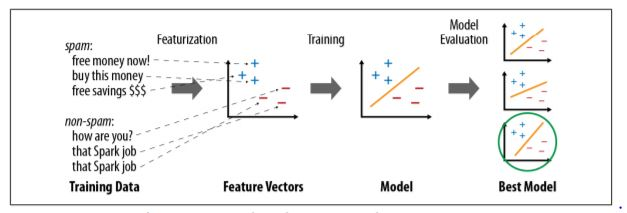
\includegraphics[scale=1]{machinelearningmllib}
	\caption{Tahapan Pembelajaran Machine Learning}
	\label{fig:machinelearningmllib}
\end{figure}
\textit{Machine learning} berupaya untuk membuat prediksi label/kelompok data berdasarkan jenis data pelatihan yang diberikan terhadap model yang dipakai. Pemodelan \textit{machine learning} termasuk ke dalam pemodelan \textit{data mining}. Jenis pemodelan machine learning terdiri dari klasifikasi, regresi, dan pengelompokan/\textit{clustering}. Seluruh jenis pemodelan \textit{machine learning} membutuhkan input berupa vektor fitur. Vektor fitur adalah nilai masing-masing atribut yang digunakan pada pelatihan data. Sebagian besar pemodelan \textit{machine learning} hanya menerima input vektor berupa data numerik untuk mewakili vektor fitur pada setiap baris data.
\\\\
\noindent Gambar \ref{fig:machinelearningmllib} adalah tahapan \textit{machine learnin}g pada Spark MLlib, berikut adalah penjelasan singkat dari masing-masing tahapan:

\begin{enumerate}

\item \textit{Featurization}\\
Setelah data telah dibersihkan dan dipilih untuk pelatihan, perlu diubah menjadi representasi numerik dalam bentuk vektor sebagai input untuk model. Proses ini disebut vektorisasi. Proses pemilihan fitur yang tepat berpengaruh terhadap hasil pelatihan.
 
\item \textit{Training}\\
Pelatihan model merupakan salah satu tahapan yang paling memakan waktu dan padat karya dalam setiap alur kerja \textit{machine learning}. Terlebih lagi, perangkat keras dan infrastruktur yang digunakan untuk melatih model sangat bergantung pada jumlah parameter dalam model, ukuran dataset, metode pengoptimalan yang digunakan, dan pertimbangan lainnya.

\item \textit{Model Evaluation}\\
Setiap model harus menjalani evaluasi kualitatif dan kuantitatif. Banyak data pelatihan yang memiliki hasil evaluasi yang sesuai terhadap kinerja model. Model tersebut harus diterapkan pada data baru. Seringkali, pemeriksaan kualitatif tentang kinerja model, diperoleh dengan referensi silang prediksi model dengan apa yang diharapkan secara intuitif, dapat berfungsi sebagai panduan apakah model bekerja sesuai harapan.
\end{enumerate}

\subsection{Tipe Data pada Spark MLlib}
Seperti yang sudah dijelaskan pada bagian \ref{sec:ml_sparkmllib}, pemodelan \textit{machine learning} menerima input berupa vektor fitur. Tipe data yang disediakan pada Spark MLlib terdiri dari beberapa jenis yaitu vektor, \textit{labeledpoint}, dan \textit{various model class}. Masing-masing tipe data pada Spark MLlib ditentukan berdasarkan jenis pemodelan yang dipilih. Contoh apabila menggunakan pemodelan \textit{clustering} akan digunakan tipe data vektor, sedangkan untuk pemodelan klasifikasi akan digunakan tipe data \textit{labeledpoint}. \textit{Various model class} digunakan untuk menyimpan hasil pemodelan yang dipilih yaitu pengelompokan/\textit{clustering} maupun klasifikasi.

\newpage
\noindent Berikut adalah penjelasan jenis tipe data pada Spark MLlib:

\begin{itemize}
\item Vektor\\
Vektor terdiri dari dua jenis yaitu vektor dense dan vektor sparse. Kelas vektor berada pada package mllib.linalg.Vectors. Berikut penjelasan singkat vektor dense dan vektor sparse:

\begin{itemize}

\item Vektor dense\\
Vektor dense adalah vektor yang menyimpan setiap nilai fitur dataset. Jumlah elemen pada vektor dense akan memiliki jumlah yang sama dengan jumlah fitur pada dataset. \\

\item Vektor sparse\\
Vektor sparse adalah vektor yang menyimpan setiap nilai fitur yang bukan nol pada dataset, sehingga jumlah elemen yang disimpan pada vektor sparse lebih sedikit dibandingkan dengan jumlah elemen yang disimpan pada vektor dense. 

\end{itemize}

\item \textit{LabeledPoint}\\
\textit{LabeledPoint} digunakan pada algoritma \textit{supervised learning} yaitu klasifikasi dan regresi. LabeledPoint terdiri dari vektor fitur dan label yang direpresentasikan dengan tipe data Double. Kelas \textit{LabeledPoint} terletak pada package mllib.regress.

\item \textit{Various Model class}\\
\textit{Various Model classes} adalah tipe data yang dihasilkan dari pemodelan \textit{machine learning}. Tipe data ini memiliki fungsi predict() untuk melakukan prediksi label dan kelompok data.

\end{itemize}

\subsection{Data Mining pada Spark MLlib}
Data mining pada Spark MLlib menggunakan tahapan pemodelan pada \textit{machine learning} yang dijelaskan pada bagian \ref{sec:ml_sparkmllib} untuk menghasilkan tabel hasil pengelompokan dan klasifikasi. Pada bagian ini akan dijelaskan parameter dari pemodelan Spark MLlib.

\subsubsection{Naive Bayes}
\label{sec:naivebayes_mllib}
\textit{Naive Bayes} menjadi pemodelan klasifikasi yang umum digunakan. \textit{Naive Bayes} dapat dilatih dengan sangat efisien karena prosesnya hanya menghitung probabilitas bersyarat masing-masing atribut dan mencari probabilitas tertinggi. \textit{Naive Bayes} memiliki parameter masukan sebagai berikut:
 
\begin{itemize}
\item \textit{randomSplit} adalah membagi training dan test data berdasarkan persentase.
\item \textit{setModelType} adalah memilih model yang tersedia (\textit{multinomial/bernoulli})
\item \textit{setLabelCol} adalah memilih jenis atribut yang menjadi label kelas.
\end{itemize}

\subsubsection{K-Means}
\label{sec:kmeans_mllib}
\textit{K-means} menjadi pemodelan pengelompokan/\textit{clustering} yang paling umum digunakan untuk mengelompokkan titik-titik data menjadi sejumlah kelompok yang telah ditentukan. \textit{K-means} memiliki parameter masukan sebagai berikut:

\begin{itemize}
\item \textit{k} adalah jumlah cluster yang diinginkan. 
\item \textit{maxIterations} adalah jumlah iterasi maksimum yang harus dijalankan.
\item \textit{initializationMode} menentukan inisialisasi centroid secara acak.
\item \textit{initializationSteps} menentukan jumlah langkah dalam algoritma \textit{k-means}.
\item \textit{initialModel} adalah menentukan nilai centroid saat inisialisasi.
\end{itemize}

\section{Scala}
\label{sec:scala}
Scala adalah bahasa pemrograman berbasi open source, dibuat oleh Profesor Martin Odersky. Scala adalah bahasa pemrograman multi-paradigma dan mendukung paradigma fungsional serta berorientasi objek. Spark ditulis dalam Scala dan karena skalabilitasnya di JVM. Pemrograman Scala adalah bahasa pemrograman yang paling banyak digunakan oleh pengembang \textit{big data} untuk mengerjakan proyek Spark. Untuk pengembangan Spark, penulisan sintaks Scala dianggap produktif untuk mengimplementasikan kode program. Pemrograman pada Scala mempertahankan prinsip keseimbangan antara produktivitas pengembangan program dan kinerja program. Pemrograman pada Scala tidak serumit pemrograman pada Java. Satu baris kode program pada Scala dapat menggantikan 20 hingga 25 baris kode Java. Karena alasan terbut, Scala menjadi bahasa pemrograman yang sangat diminati untuk melakukan pemrosesan \textit{big data} pada Spark.

\section{Scala Swing} 
Scala Swing adalah program berbasis \textit{Graphical User Interface} (GUI) sehingga memiliki perbedaan dengan program Spark yang dieksekusi dengan terminal. Scala Swing bertujuan untuk memberi tampilan program sehingga hasil program diharapkan menjadi lebih interaktif. Scala menyediakan akses langsung terhadap kelas GUI pada Java menggunakan \textit{library} Scala Swing.  Dengan menggunakan Scala, penggunaan Scala Swing dapat memenuhi kebutuhan perancangan \textit{User Interface} melalui berbagai macam komponen GUI pada umumnya. Gambar \ref{fig:swing_example} adalah contoh implementasi GUI sederhana pada Scala Swing.

\begin{figure}[H]
	\centering
	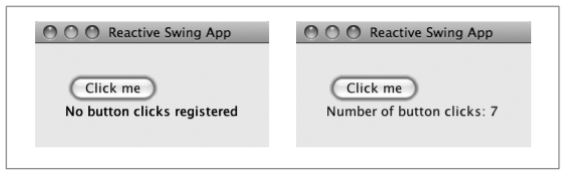
\includegraphics[scale=0.9]{swing_example}
	\caption{GUI Sederhana pada Scala Swing}
	\label{fig:swing_example}
\end{figure}


\subsection{Panel dan Layout}
\textit{Panel} adalah tempat untuk menampilkan semua komponen GUI dengan beberapa aturan tata letak yang harus dipenuhi. Salah satu bagian tersulit pada perancangan aplikasi berbasis GUI adalah mengatur penempatan layout dengan benar. \textit{Layout} terdiri dari beberapa komponen GUI seperti \textit{Frame, Panel, Label} atau \textit{Button}. Masing-masing komponen GUI pada \textit{layout} memiliki nilai properti sendiri (warna, ukuran, posisi) yang dapat diatur secara manual.

\subsection{Handling Event}
\textit{Handling event} adalah perkerjaan yang dilakukan masing-masing komponen. Komponen akan menerima aksi langsung dari pengguna aplikasi. Mekanisme ini dikenal sebagai \textit{handling event}, yang dieksekusi ketika suatu peristiwa terjadi. \textit{Handling event} memiliki \textit{listener}. \textit{Listener} adalah sebuah komponen memberi tahu sebuah aksi kepada komponen tertentu. \textit{Listener} harus dibuat untuk masing-masing objek \textit{handling event}. 

\section{Format File}
Spark menyediakan cara sederhana untuk mengambil dan menyimpan file data dalam ukuran yang besar berdasarkan format \textit{file} tertentu. Format ini dapat berupa data yang tidak terstruktur seperti teks, hingga data semi-terstruktur seperti JSON, dan data terstruktur seperti CSV. Gambar \ref{fig:format_file} menunjukan format file yang dapat ditangani oleh Spark yaitu \textit{JSON, Text, Sequence, Object}, dan \textit{Hadoop Input Output Format}.

\begin{figure}[H]
	\centering
	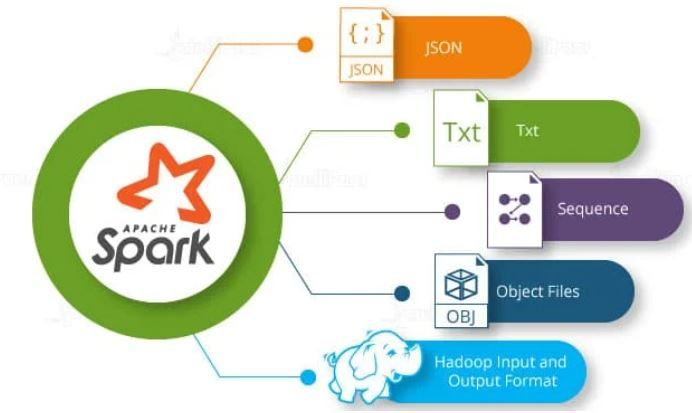
\includegraphics[scale=0.5]{format_input}
	\caption{Format File pada Spark}
	\label{fig:format_file}
\end{figure}

\subsection{Text}
\textit{Text} adalah standar yang umum format \textit{file} yang digunakan untuk mengambil data input dan menyimpan hasil pengolahan data pada program Spark. Ketika Spark memuat sebuah file \textit{text} sebagai RDD, maka setiap baris data pada \textit{file text} tersebut diubah menjadi elemen pada RDD. Berikut adalah contoh penggunaan format \textit{text} pada Spark:

\begin{itemize}

\item Mengambil \textit{file} Text: cara ini dipakai untuk mengambil data input dalam format teks pada sebuah direktori. Fungsi untuk mengambil file teks pada Spark adalah \textsf{textFile()}. Fungsi textFile() menerima parameter direktori pada komputer lokal/hdfs tempat file text tersebut disimpan.

\item Menyimpan \textit{file} Text: cara ini dipakai untuk menyimpan hasil pengolahan data dalam format teks pada sebuah direktori. Fungsi untuk menyimpan hasil pengolahan data dalam file teks pada Spark adalah \textsf{saveAsTextFile()}. Fungsi tersebut menerima parameter direktori lokal/hdfs tempai file text tersebut akan disimpan

\end{itemize}

\subsection{CSV/TSV}
\label{theory:csv}
\textit{Comma Separated Values} (CSV) menjadi format yang sangat umum digunakan untuk menyimpan nilai pada tabel data. CSV menyimpan data untuk setiap baris data yang nilainya dipisahkan oleh tanda koma. \textit{Tab Separated Values} (TSV) memiliki penyimpan yang hampir mirip dengan CSV. TSV memiliki nilai yang dipisahkan oleh tanda tab. Berikut adalah contoh penggunaan format CSV dan TSV pada Spark:

\begin{itemize}

\item Mengambil \textit{file} CSV: cara ini dipakai untuk mengambil data input dalam format CSV pada sebuah direktori. Fungsi untuk mengambil file CSV pada Spark adalah \textsf{textFile()}. Fungsi textFile() menerima parameter direktori pada komputer lokal/hdfs tempat file text tersebut disimpan. 


\item Menyimpan \textit{file} CSV: cara ini dipakai untuk menyimpan hasil pengolahan data dalam format CSV pada sebuah direktori. Fungsi untuk menyimpan hasil pengolahan data dalam file CSV pada Spark adalah \textsf{write.csv()}. Fungsi tersebut menerima parameter direktori lokal/hdfs tempai \textit{file CSV} tersebut akan disimpan.


\end{itemize}


